%!TEX root = ../main.tex

\chapter[Gradual Accumulation of Modification]{Gradual accumulation of modification in children's literature}\label{chp:red-riding-hood}

\chapterprecishere{\filcenter``Pas op! Je kent het verhaal toch?''}{Caroline Ellerbeck}{Roodkapje}

\section{Introduction}\label{sec:introduction}

Many of the stories that occur in children's literature have an interesting property in common with folktales: they are retold and adapted. Clearly, folktales -- especially those from oral culture -- depend on retellings in order to secure their survival in culture. Each retelling of a story forms the endpoint of a chain of retellings. The continuation of the chain of retellings, or in other words, the lifespan of a story, depends on whether the story will be further retold; if not, its lifespan ends and the story becomes extinct. As \citeauthor{burkert:1982} aptly describes: ``A tale becomes traditional not by virtue of being created, but by being retold and accepted; transmission means interaction [...]''\autocite[2]{burkert:1982}. When it comes to stories in children's literature, which exist mostly in printed or electronic form and, as such, substantially differ from oral folktales, it could be argued that their survival depends first and foremost on the conservation of their printed or electronic records (e.g.\ in library collections, on a bookshelf or on the Internet). However, scholars have noted that children's stories are retold and adapted as well, and it is stressed that, like oral folktales, children's stories \emph{need} to be recurrently adapted to secure their position in culture\autocite{stephens_mccallum,collins_ridgman,geerts:2014}. This is due to the fact that retellings in children's literature have important cultural functions, one of which is to ``initiate children into aspects of a social heritage, transmitting many of a culture's central values and assumptions and a body of shared allusions and experiences''\autocite[3]{stephens_mccallum}. Since a culture's central values and ideologies are never fixed but always in transition, adaptations and transpositions are necessary to maintain the relevance of stories for new audiences in changing historical contexts\autocite{collins_ridgman}. 

The consequence of considering a story as a \emph{re}-telling is that it is positioned in relation to one source or even multiple source texts. In line with \citeauthor{stephens_mccallum}, I will refrain from using the term `source text' and apply the more neutral term `pre-text'\autocite{stephens_mccallum}. Oral folktales are generally derived from pre-texts from the immediate previous generation\autocite[See][]{rubin:1995}, and each retelling produces a slightly (or very) different story, due to e.g.\ subconscious factors such as memory capacity\autocite[Cf.][]{bartlett} or conscious factors such as the creativity of the storyteller\autocite[Cf.][]{boyd:2009}. In other words, the oral transmission of folktales is best described as a process of `gradual accumulation of modifications': oral folktales ``are transmitted from individual to individual and generation to generation via social learning mechanisms such as imitation, thus forming lineages of similar traits''~\autocite[90]{mesoudi:2011}, with each individual potentially introducing modifications which may be adopted and further transmitted in the next retelling.  

When it comes to the transmission of literary texts and children's literature (rather than oral folktales), we may be inclined to believe that transmission is not `gradually accumulating', but that adaptations in retellings are derived from some original (printed) text or `urtext' rather than from younger retellings. This would mean that all retellings of, for instance, ``Red Riding Hood'' are second generation stories that are most likely immediately derived from the version by the Brothers Grimm. However, \citeauthor{stephens_mccallum} hypothesize that:
\begin{quotation}
    \noindent A familiar fairy tale such as \emph{Cinderella} may derive from Perrault's version, or the Disney film, or British pantomime tradition, but is more apt to borrow freely from amongst these and from versions of them circulating orally. Even where there is a strong pre-text such as Perrault, retellers are most likely to use intermediate versions--to produce a retelling of a retelling.~\autocite[4]{stephens_mccallum}
\end{quotation}
In other words, these `retellings of retellings' in children's literature too form a network (rather than a tree) of `intermediate' story versions without a clear `root story' from which all subsequent versions have supposedly sprang. From a theoretical perspective, the effort spent to identify such a `first telling', which has been one of the main occupations of many folklore scholars in the \nth{19} century and scholars of the `Finnish' or historical-geographic school, is questionable at best\autocite[For a more recent example of such effort, see][]{tehrani:2013}. Retellings of \emph{Cinderella} are influenced by intermediate retellings of the story and the alleged `original' written by Perrault is no different. Perrault's story also represents some intermediate state, because his version is guided by what \citeauthor{frank:2010}, influenced by Bourdieu, calls a \emph{narrative habitus}:
\begin{quote}
    Narrative habitus is a disposition to hear some stories as those that one ought to listen to, ought to repeat on appropriate occasions, and ought to be guided by. [\ldots] [N]arrative habitus involves a \emph{repertoire} of stories that a person at least recognizes and that a group shares. These stories are known against an unseen background of all the stories that person does not know and stories that do not circulate within any particular group.\autocite[53]{frank:2010}
\end{quote}
Perrault's narrative habitus was formed by -- obviously against the background of a much broader literary context -- fairy tales written by (mostly female) writers such as Marie-Jeanne L'Héritier, Marie-Catherine d'Aulnoy and Jean de La Fontaine\autocites[76]{warner:1995}[44]{zipes:2012}. Perrault had a `Mother Goose' of his own, so to speak\autocite[44--45]{zipes:2012}. Stories are dependent on other texts, for which narratologists use the term \emph{intertextuality}. \citeauthor{frank:2010} prefers the term \emph{resonance} -- a term that emphasizes that intertextuality can be a personal experience -- and describes stories as ``textures of resonance''\autocite[37]{frank:2010}. As it turns out ``[i]t is quite difficult to invent a tale; even a new creation will inevitably merge with a stream of tales heard before, and thus become a variant of what has already been around''\autocite[70]{burkert:1996}. The quest for a `first telling' might seem to be a hopeless and theoretically unsound endeavor; determining \emph{the} pre-text(s) of a retelling is not a trivial task either. We can unequivocally select a pre-text or group of pre-texts for merely a handful of retellings; most are indeterminate for which no decisive answer can be provided. Nevertheless, however precisely or imprecisely, retellings are based on pre-texts and some pre-texts are more likely to have formed a source of inspiration for a particular retelling than others.

The aim of the present chapter is to investigate this simple, yet crucial hypothesis of \citeauthor{stephens_mccallum}, which holds that retellers of children's literature most likely base their retelling on `intermediate retellings'. What is meant by such intermediate retellings, however, may cover an indeterminate and considerably large time span. As such, this study aims to come to a more precise understanding of what is meant by `intermediate'. 

In its attempt to determine whether retellings in children's literature are based on intermediate versions or urtexts, and whether the transmission of children's literature can be characterized as a `gradual accumulation of modifications', the present study can be situated in a large body of research that investigates transmission of cultural traits and cultural evolution. Mesoudi sets out the sufficient conditions to consider cultural change as an evolutionary process, being (i) variation, (ii) competition (differential fitness), and (iii) inheritance~\autocite{Mesoudi:2009hx,mesoudi:2011}. In children's literature, variation exists in the sense that multiple retellings of a story exist simultaneously, which may differ on a concrete level (different wordings, character names, etc.) or a more abstract level (story elements, plot structure, cultural framing, etc.). Competition, then, is the result of certain limitations that go hand in hand with culturally acquired information: even if all existing retellings of a story are available to a reteller, this reteller can only produce \emph{one} retelling at a time. This new retelling may inherit traits of multiple existing story versions, but it is impossible to simultaneously produce (or retell) all existing versions at the exact same time. Thus, the theoretical consequence is that each time an author engages in producing a retelling, (all parts of) existing retellings are in competition to be selected as the new version's pre-text. The question is, then, why certain existing retellings are more likely to function as a new version's pre-text than others, or, in other words, what determines a retelling's `differential fitness'. 

In the cultural evolution research program, it has been suggested that such fitness of cultural variants can be generated by an interaction of various psychological, social, and ecological processes.\autocites[See e.g.][]{Henrich:2008}[Henrich et al.'s account is compatible with ecological perspectives on cultural change, such as][]{mark:1998,lieberson:2000,venrooij:2015}[For a recent discussion of the notion of `cultural fitness', see][]{ramsey:2015} The focus of this study, however, is to examine the extent to which age-dependent selection processes generate differential fitness among existing retellings -- or, in other words, whether intermediate retellings have a selection advantage over other retellings. If no such preference for intermediate retellings exists, authors may produce a retelling on the basis of some original text or sample their base material from a uniform distribution over all previous retellings (i.e.\ a modern retelling is just as likely based on a story from the immediate previous year as on a story from $n$ years back in time). In both cases, I am inclined to believe that the process through which stories in children's literature are retold cannot be conceived as gradually accumulating. I thus make the following prediction: if the evolution of stories in children's literature is a gradual accumulation of modifications, retellings are generally derived from versions in temporal proximity. 

Because it would be too big a topic to present an in-depth study of evolutionary change in children's literature at large within the scope of this chapter, I restrict this study to a single case, namely, the evolution of the world's biggest iconic fairy tale: ``Red Riding Hood''. No story has been retold, reinterpreted, recontextualized and reconfigured as often as the story about the little girl in red who meets a wolf in the forest\autocite{zipes:1993,beckett:2002,beckett:2008}. Currently, the misconception exists that fairy tales for children -- especially those written by the Brothers Grimm -- have been frozen in time and turned into static cultural artifacts. A single comparison between the version of ``Red Riding Hood'' by the Brothers Grimm and any of the modern retellings listed in \citeauthor{beckett:2002}'s \emph{Recycling Red Riding Hood} or in her anthology of international retellings furnishes all the proof that is needed to arrive at quite the opposite conclusion\autocite{beckett:2002,beckett:2014}. \citeauthor{beckett:2014} speaks of Red Riding Hood as an ``inveterate globetrotting'' girl\autocite{beckett:2014}. Indeed, the world-wide number of retellings is so vast that a complete account of the evolution of the story is completely beyond comprehension. I therefore further restrict the object of study by concentrating on the evolution of Dutch retellings of ``Red Riding Hood'' within a timespan of more than two centuries.

Applying cultural evolution theory and methods to historical story transmission is not unprecedented. In particular, the current study is reminiscent of recent research carried out by \citeauthor{tehrani:2013} who applies phylogenetic methods to study cross-cultural relationships among retellings of ``Red Riding Hood''.\autocite{tehrani:2013} Crucially, while building upon important methodological insights from \citeauthor{tehrani:2013}, the current study differs in terms of data, methods and objectives. First, the large-scale collection of Dutch ``Red Riding Hood'' retellings employed in this study (cf.\ Section \ref{sec:data}) allows for a more fine-grained tracking of the progression and evolution of the story through time. Second, the approach presented here is more thoroughly embedded in literary theory on retelling stories\autocite[e.g.][]{stephens_mccallum,zipes:1993,beckett:2002,sanders:2006,hutcheon:2013} while at the same time positions itself explicitly and extensively in dialog with the cultural evolution research program\autocite{sforzafeldman:1981,boyd_richerson:1985,mesoudi:2011}. Finally, whereas \citeauthor{tehrani:2013}'s goal is phylogenetic reconstruction, the present study is aimed at obtaining a better understanding of specific micro-evolutionary mechanisms underlying story transmission and change.

The remainder of the chapter is structured as follows. I start with a brief history of retellings of ``Red Riding Hood'' in Section \ref{sec:rrh}. I then proceed with a description of the corpus compiled for this study (Section \ref{sec:data}). Subsequently, I provide a detailed account of the data annotations (Section \ref{sec:annotations}) followed by a section about the computational and statistical methods used (Section \ref{sec:methods}). After presenting the results in Section \ref{sec:results}, I conclude with a discussion of the main findings of this study against the broader background of cultural evolution.

\section{A Brief History of Red Riding Hood}\label{sec:rrh}

Girl, forest, wolf. Three words that immediately bring the story of ``Red Riding Hood'' to mind. The girl with the red cap has been associated with myths about the sunrise and sunset\autocite[18]{zipes:1993}, was the ``first love''\autocite[xv:xvi]{beckett:2002} of Charles Dickens, who wished he could have married her -- ``I should have known perfect bliss'' -- and is what \citeauthor{orenstein:2002} calls ``the age-old star of bedtime drama''\autocite[3]{orenstein:2002}. The tale has been told in poems, short stories, picture books, theater, comics and cartoons, video games, film, adult literature, advertisements, and even entire operas are devoted to the fortunes of the girl in red\autocite{beckett:2008,zipes:1993}. As Jack Zipes writes in his seminal book, \emph{The Trials and Tribulations of Little Red Riding Hood}, it is ``the most popular and certainly the most provocative fairy tale in the Western world''\autocite[343]{zipes:1993}. Everyone knows ``Red Riding Hood''. But do we really?

\subsection{Perrault's Rape Story}
The first literary version of the tale, \emph{Le petit Chaperon rouge}, written by Charles Perrault in his 1697 collection \emph{Contes du temps passé avec moralités}, is a retelling based on oral versions\autocite[20]{zipes:1993}. Perrault produced a truncated version and removed many elements dominant in oral tradition. However, some of those elements did survive the popularity of Perrault's version. In one oral retelling recorded around 1885\autocite[21-23]{zipes:1993}, a little girl, after meeting with the wolf in the forest, is tricked into eating the flesh and drinking the blood of her grandmother (after which she is scolded by a little cat: ``Phooey!... A slut is she who eats the flesh and drinks the blood of her granny.''). After an elaborate undressing scene, the girl manages to escape from the wolf by saying that she has ``got to go badly''. The wolf proposes to do it in bed, but the girl refuses. Under the condition that she wears a woolen rope around her foot, the wolf allows her to leave the house. Once outside, she ties the rope to a tree and flees. 

\begin{figure}[t]
    \centering
    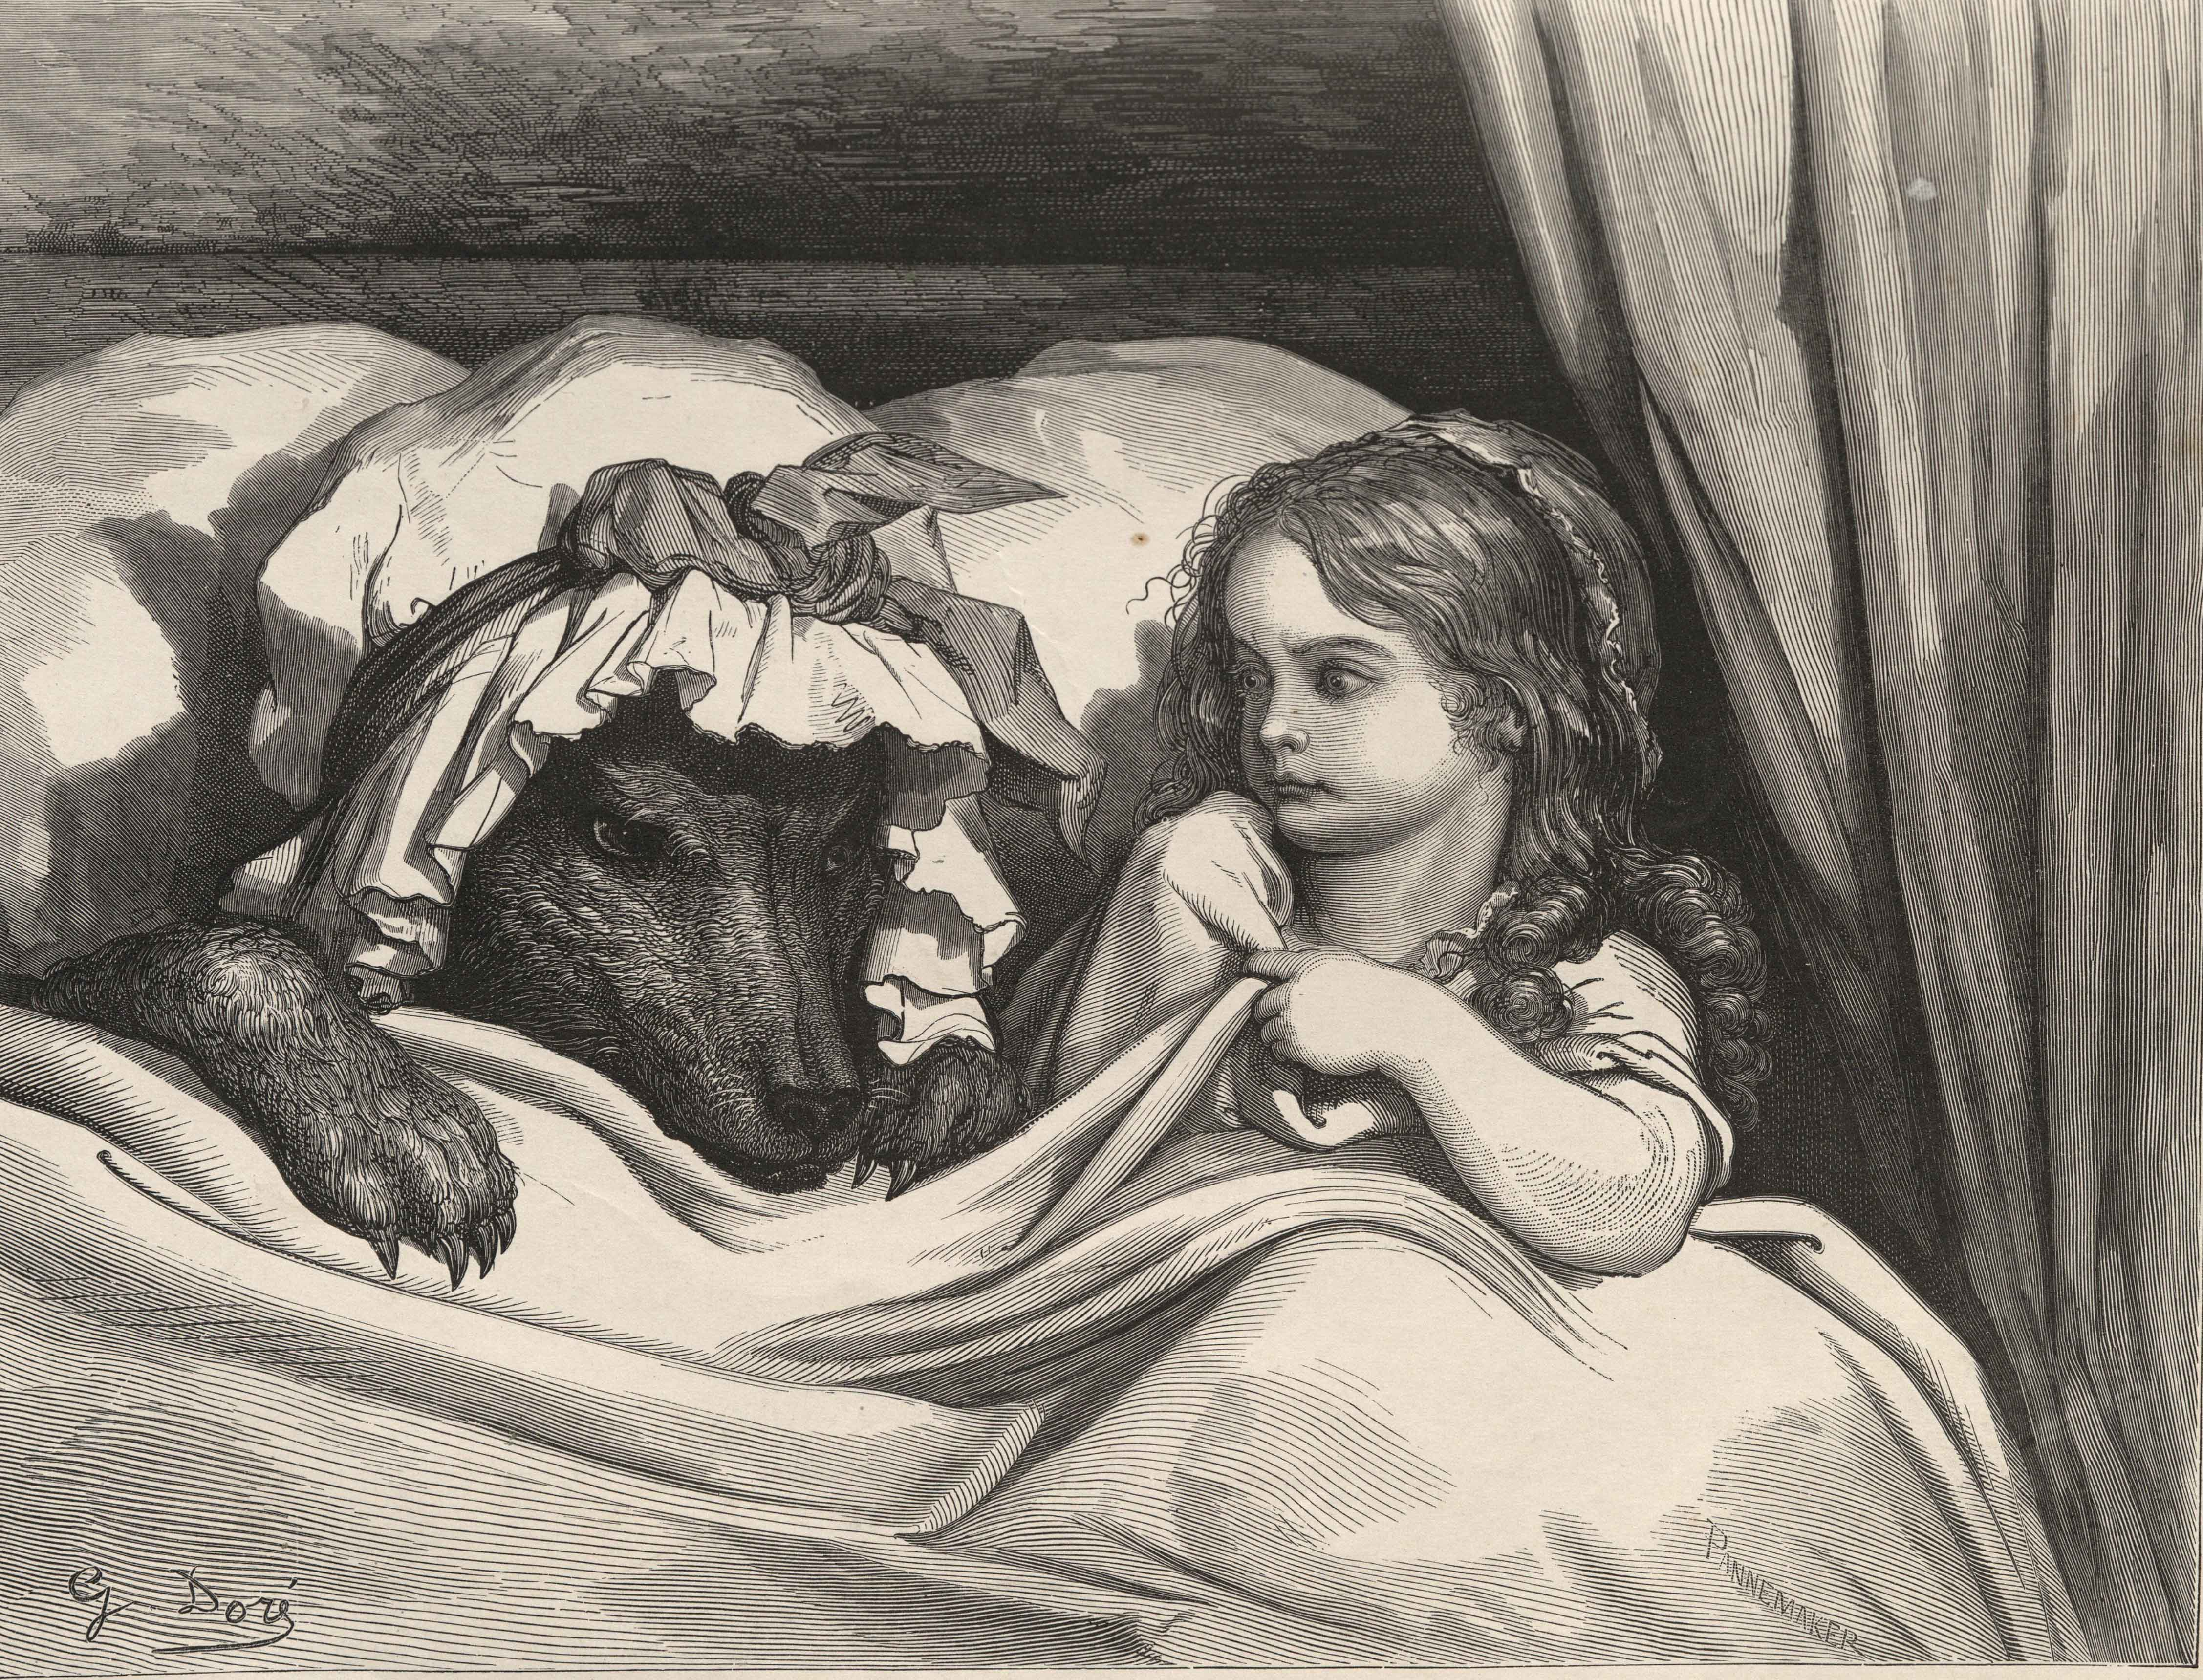
\includegraphics[width=\textwidth]{images/dore}
    \caption{\emph{Little Red Riding Hood}, by Gustave Doré (1883).}
    \label{fig:dore}
\end{figure}

Most of these elements are either removed or refined in Perrault's literary version. In \emph{Le petit Chaperon rouge} Red Riding Hood is devoured by the wolf, and unlike in versions of the story children know today, there is no salvation. Perrault's collection of tales is dedicated to Elisabeth Charlotte d'Orleans, Louis XIV's niece and many elements of the story implicitly or explicitly -- especially in the rhyming moral at the end -- refer to court of the Sun King. As \citeauthor{beckett:2008} makes clear: ``Perrault turns the oral tale into a parable, particularly adapted for use at the court of Versailles, that warns young ladies to be aware of suave and debonair two-legged wolves who would sweet-talk their way into their beds and ruin their reputations''\autocite[13]{beckett:2008}.

Perrault's version is replete with sexual innuendos, most prominently in the ending moral, but also in the preceding narrative (e.g.\ ``What big arms you have, grandmother!''). \citeauthor{zipes:1993} makes a strong case that Perrault transformed a once hopeful oral tale into an aggressive and violent story about a helpless girl who is to be held responsible for her own rape\autocite{zipes:1993}. The etching by Doré from 1867 in Figure \ref{fig:dore} illustrates Zipes' thesis. It shows the image of a little girl, seemingly oblivious of the wolf's intentions, who covers herself with the bed linen and gives the wolf a seductive look. She appears to have no fear, suggesting that ``if she were not gullible and disobedient, she could prevent the rapacious wolf from carrying out his designs''\autocite[39]{zipes:1993}.

\begin{figure}
\centering
\includegraphics[width=\textwidth]{images/pennycatch}
\caption{\emph{De vertelling van Roodkapje}, Erve H. Rynders, 1831 -- 1854.}
\label{fig:pennycatch}
\end{figure}

The oldest Dutch translation in my corpus of ``Red Riding Hood'' retellings (see section \ref{sec:data}) is entitled \emph{De vertelling van Roodkapje} (`The tale of Little Red Riding Hood') and stems from 1781. This version and most Dutch retellings of ``Red Riding Hood'' in the \nth{19} century adhere to the plot structure of Perrault's story. The suggestive rhyming moral, however, is either set aside or altered by many authors. It is interesting to note that many retellings bear the word \emph{nieuw} (`new') in their title as in the anonymous 1818 version \emph{De Nieuwe Geschiedenis van Roodkapje} (`The new history of Red Riding Hood'). As \citeauthor{beckett:2002} remarks, this reminds us ``that retellings have always been an attempt to rejuvenate the tale for a contemporary audience''\autocite[xvi]{beckett:2002}. Many of the oldest versions of ``Red Riding Hood'' in the Netherlands were published as so-called pennycatch prints. Pennycatch prints were the cheapest illustrated printed material -- for one or a few pennies -- and report on important events or tell popular stories such as ``Red Riding Hood'' on a single sheet of paper, slightly larger than the current A3-format. Figure \ref{fig:pennycatch} provides an example one of the pennycatch prints in the collection. 

\subsection{Grimms' Story of Discipline}
The second classic retelling of ``Red Riding Hood'' is the one by the Brothers Grimm, \emph{Rothkäpchen}, originally published in 1812 in the collection \emph{Kinder- und Hausmärchen}. The most striking change made by the Brothers Grimm is the rescue scene of Little Red Cap by a hunter. Little Red Cap may not be killed, yet it could be argued that the Brothers Grimm emphasize the image of a naive and helpless girl even more\autocite[32]{zipes:1993}. In contrast with the oral versions, Little Red Cap is unable to save herself and is dependent on the protection of a father figure. The Brothers Grimm have reworked and revised their collection several times in an attempt to adapt the story to fit the emerging Biedermeier image of a child: Little Red Cap must show obedience and good behavior\autocite[32--37. For an automatically generated alignment of the seven versions published by the Brothers Grimm, see \texttt{http://fbkarsdorp.github.io/grimms}.]{zipes:1993}. The emphasis on good behavior is apparent from the added cautionary scene in which Little Red Cap is warned about the dangers of talking to strangers, straying from the path or lingering in the woods. In the 1850 and 1857 edition, the Brothers Grimm stress the importance of good manners when the mother commands the girl: ``Und wenn du in ihre Stube kommst, so vergiß nicht guten Morgen zu sagen und guck nicht erst in alle Ecken herum.''\footnote{`And when you enter her parlor, don't forget to say `Good morning', and don't peer into all the corners first.'} Little Red Cap promises to be obedient, but she is not, and therefore she needs to be punished. At the end of the story, Little Red Cap is aware of her disobedience and concludes that she is to be held responsible for her fate. Some Dutch retellers have emphasized this lesson using a more elaborate moral, as in the version by Simon Jacobus Andriessen (1880): ``Die kwaad doet, kwaad ontmoet! en: Wie niet hooren wil, moet voelen!'' (`He that mischief hatches, mischief catches!' and: `He that will not be counseled cannot be helped!'). 

\begin{figure}[t]
    \centering
    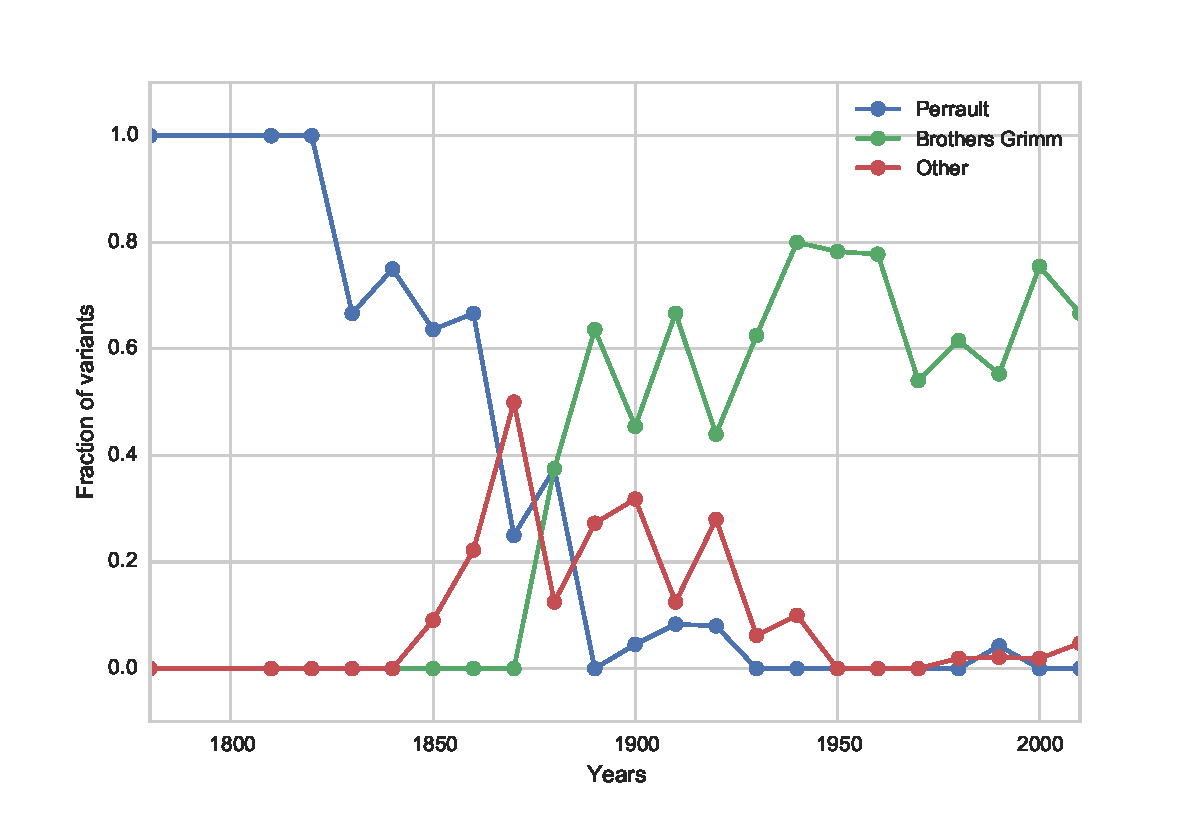
\includegraphics[width=\textwidth]{images/battle}
    \caption{Population plot showing the fraction of retellings per decade of ``Red Riding Hood'' classified as a version of either Perrault, the Brothers Grimm, or `other'.}
    \label{fig:battle}
\end{figure}

Perrault's tale and the retelling of the Brothers Grimm have been popular in the Netherlands. However, the number of retellings that showed signs of being influenced by the Brothers Grimm directly after \emph{Kinder- und Hausmärchen} was published in 1857 is rather low. Over the years the numbers gradually increased before it `took off' in the 1890s and ``it virtually dwarfed Perrault's version''\autocite[36]{zipes:1993}. Figure \ref{fig:battle} visualizes the competition between Perrault and the Brothers Grimm from the late \nth{18} century to the early \nth{21} century in the Netherlands. The plot shows for each decade from 1780 to 2010 the fraction of retellings that can be classified as a version derived from either Perrault, the Brothers Grimm or `other'. A retelling is classified as a Perrault version if both the grandmother and the girl are eaten by the wolf and they are not rescued. A version counts as a retelling of the Brothers Grimm if, after being swallowed, both the grandmother and the girl are saved from the wolf's belly. The `other' group shows the fraction of versions in which the grandmother is devoured (without being rescued) while the girl is saved before the wolf is able to lay a hand on her. Without more information about the rest of the narrative, it is hard to say whether these versions adhere to the Perrault or to the Grimm paradigm. They do fit the trend of `Victorian censorship' of the \nth{19} century in which scenes considered to be too cruel or too sexual were replaced. 

\begin{figure}
\centering
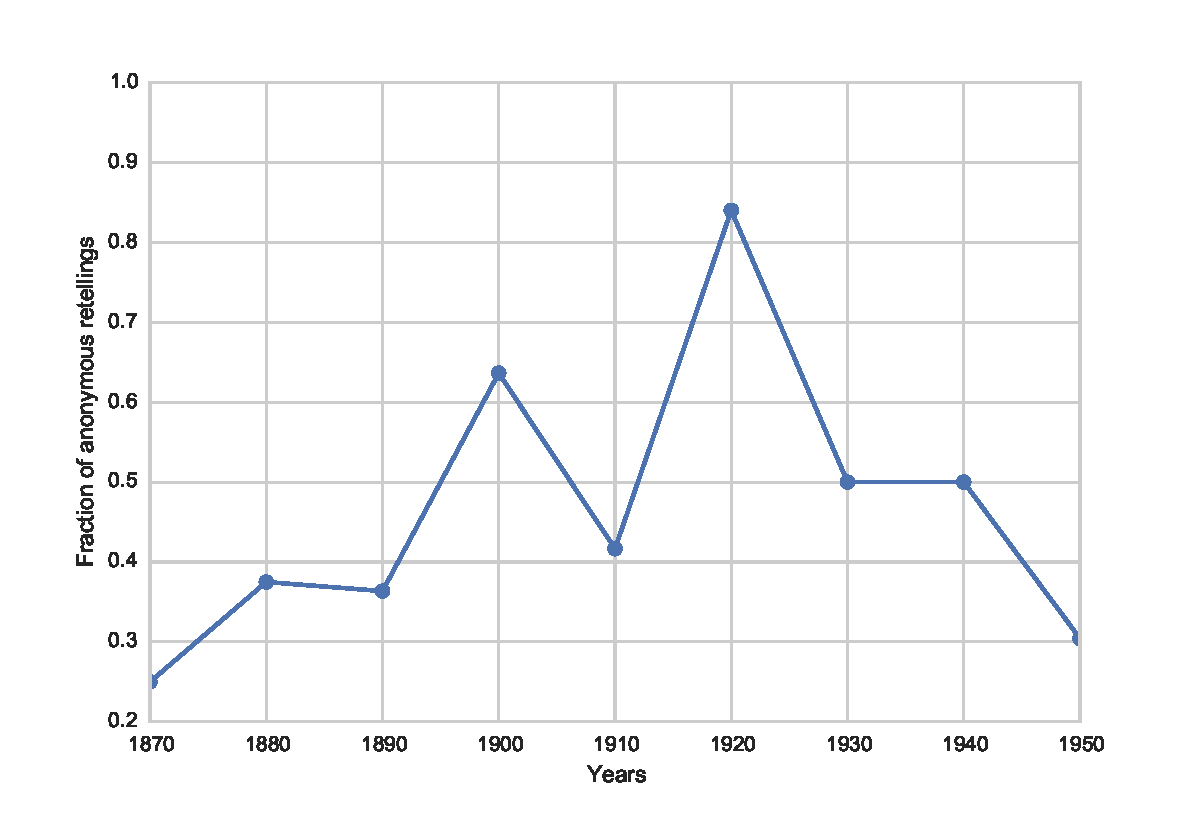
\includegraphics[width=\textwidth]{images/anonymous}
\caption{Fraction of anonymous (versus authored) retellings of ``Red Riding Hood'' over the period 1870 -- 1950.}
\label{fig:anonymous}
\end{figure}

It is interesting to observe that the explosive burst of retellings within the Grimm paradigm is followed by a `stabilizing' period at the beginning of the \nth{20} century in which no radical changes to the story are made. As illustrated by Figure \ref{fig:anonymous}, this is also a period in which a large number of anonymous retellings of ``Red Riding Hood'' were published, possibly to evoke an image of authenticity as a tale from oral history. Furthermore, quite a number of retellings position themselves explicitly in relation to either Perrault or the Brothers Grimm. An example from my corpus appeared in the collection \emph{Sprookjes Van Moeder De Gans} (`Fairy tales by Mother Goose') written by Christine Doorman (1916). Although the title of the collection refers to Perrault, the story of ``Red Riding Hood'' more closely resembles the plot structure of the Brothers Grimm with its reassuring rescue scene. The beginning of the \nth{20} century might be epitomized as a period in which the fairy tale becomes increasingly generic and autonomous, not bound to a particular author but residing in the collective imagination. In this context, Soriano aptly suggests that the fairy tale has become a text ``without a text'' and a text ``without an author''\autocite[cited in][xvii]{beckett:2002}.

\subsection{Time for Change}
We might hypothesize that within the context of a literary environment in which there is a strong tradition of the story, yet it is not linked to a specific author, retellers are able to engage more freely with the material\autocite{beckett:2002}. Starting from the 1940s but especially in recent decades, an increasing number of retellings expose radical innovations, aesthetic experimentation and intertextual references. Because of their limited exposure to cultural heritage, children are generally assumed to be less competent in decoding these intertextualities. \citeauthor{beckett:2002} argues that in the case of ``Red Riding Hood'', authors \emph{can} use these sophisticated narrative strategies, because they can safely assume children know at least some version of the story, which provides them with the necessary decoding tools\autocite{beckett:2002}.

\begin{figure}
    \centering
    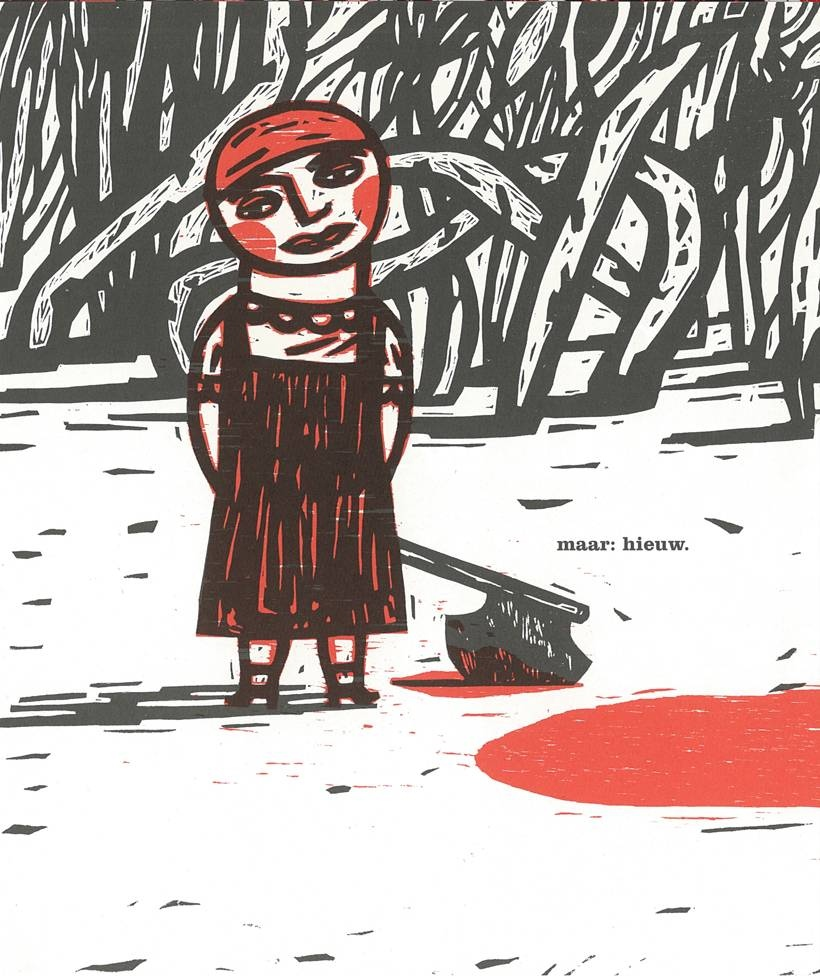
\includegraphics[width=\textwidth]{images/vendel_wolfdood}
    \caption{\emph{Rood Rood Roodkapje}, by Edward van de Vendel; illustration: Isabelle Vandenabeele (2003).}
    \label{fig:red-red}
\end{figure}

After World War II, the story of ``Red Riding Hood'' branched off in too many directions to enumerate in this overview. \citeauthor{zipes:1993} distinguishes three major branches: (i) retellings in which ``Red Riding Hood'' becomes increasingly independent, (ii) versions that rehabilitate the wolf and/ or tell his version of the story and (iii) stories that stand out with respect to their aesthetic experimentation\autocite[59]{zipes:1993}. I discuss an example from each of these branches to illustrate some of the radical changes the story has undergone.

\subsubsection*{Rood Rood Roodkapje}
The retelling \emph{Rood Rood Roodkapje} (`Red Red Red Riding Hood') by the Dutch author Edward van de Vendel with illustrations by the Flemish illustrator Isabelle Vandenabeele, is an exciting example of a retelling in which Red Riding Hood has become self-reliant\autocite{vendel:2003}. Vandenabeele makes use of a drawing style that is reminiscent of the etchings by Gustave Doré, yet much coarser and only in the colors gray, black and red. Red Red Red Riding Hood only wishes for red things, red clothes, red juice, red carpet, red pillows on her bed. She had to choose her own name -- the reversal of a dominant motif in ``Red Riding Hood'', which is iconic of her more independent status. All her wishes are red, but her days are gray, because she has to walk the gray muddy paths everyday to her gray grandmother. Then one day, she encounters something black\ldots The Wolf. By accident she shows the Wolf the way to her grandmother. The Wolf immediately spurts to her grandmother and devours her with a terrifying howling sound. Determined to make up for her mistake, Red Red Red Riding Hood follows the Wolf to her grandmother's house. No, this time there is no howling 

\begin{quotation}
\noindent
{\fontsize{2cm}{1em}\selectfont%
grwarwah\vspace{0.5cm}\\
briaaauwah\vspace{0.5cm}\\
hgroing\vspace{0.5cm}\\
raaaaaaaaa\vspace{0.5cm}\\}
\noindent {\scriptsize But: chop.}
\end{quotation}

After the restrained slaying scene, we see a calm girl with a somewhat subdued and contemplative look on her face, holding a bloody ax, while the blood flows from her grandmother's doorway (cf.\ Figure \ref{fig:red-red}). Content with the thought that she never has to visit her grandmother again, Red Red Red Riding Hood imagines all the red things she can do in her life. As in the old French oral version of the story in which ``Red Riding Hood'' outwits the wolf, Van den Vendel and Vandenabeele present a girl who is no longer timid, innocent or powerless, but rather fearless, determined and self-assured.

\begin{figure}[t]
    \centering
    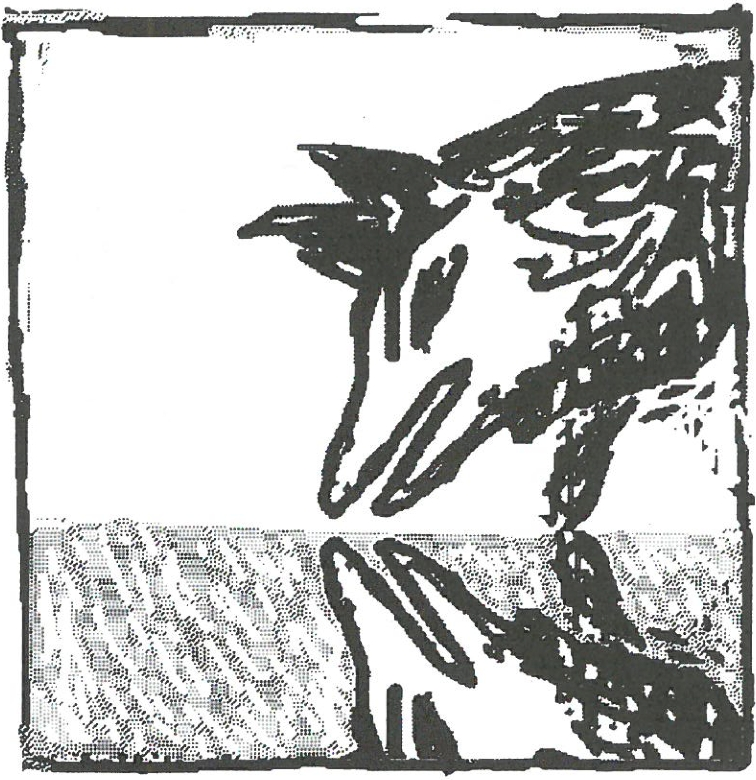
\includegraphics[width=\textwidth]{images/Waterwolf}
    \caption{\emph{De Wolf die tegen water praatte}, by Imme Dros; illustration: Henricus Geelen (1991).}
    \label{fig:waterwolf}
\end{figure}

\subsubsection*{De Wolf die tegen water praatte}
At an abstract level, the story \emph{De Wolf die tegen water praatte} (`The Wolf who talked to water') by the Dutch author Imme Dros, closely resembles traditional retellings of ``Red Riding Hood'': (i) A girl meets a wolf in the forest, (ii) the wolf swallows both the girl and her grandmother, (iii) they are rescued by a hunter, and (iv) the wolf, filled with stones, drowns in the water\autocite{dros:1991}. The perspective of the story, the ordering of the different plot elements and especially the meaning attributed to these elements, however, is completely different. The story, reminiscent of Ovid's \emph{Narcissus}, tells us about the wolf Noordenloos (`Northless') whose only friend is his reflection in the water (cf.\ Figure \ref{fig:waterwolf}). The lonely Noordenloos wishes to return to his former wolf pack in the North together with his imaginary friend Waterwolf. One day, after having a conversation with Waterwolf, Noordenloos meets a girl, who asks for directions to her grandmother's cottage. Following the traditional plot structure, the wolf arrives at grandmother's house before Red Riding Hood does, swallows the grandmother, tricks Red Riding Hood using his famous disguise, and finally, gobbles her up. However, unlike in most traditional retellings, the primary reason for eating Red Riding Hood and her grandmother is not to stave off hunger, but serves to strengthen the wolf for his escape from loneliness to the North. Yet, he only manages to join his family in the North in his own imagination at the moment of his -- metaphorically described -- death: he was happy. By approaching the story from the wolf's perspective, Dros transforms the wolf from being primarily `Big and Bad' into a real character with a soul, feelings, thoughts and desires. 

\subsubsection*{Roodkapje en de zeven geitjes}

The experimental retelling written by Ivo de Wijs with illustrations by Alfons van Heusden (\citeyear{wijs:1994}) diverges radically from the tradition, both in form and in content. The story is part of a collection entitled \emph{Roodkapje en de zeven geitjes} (`Red Riding Hood and the Seven Kids'). This rather unusual juxtaposition of characters from two famous fairy tales serves to emphasize the bricolage nature of the stories to come. Each story in the book tells three different versions of a story. On each page, supposedly aligned fragments of the three versions are placed side by side in three columns, each with its own distinctive typography. The reader is supposed to read all three columns before moving on to the next page (see Figure \ref{fig:dewijs} for a translation of the first paragraphs of each version).

\begin{figure}
{
\centering
\begin{tabular}{>{\raggedright}p{0.3\textwidth} >{\raggedright}p{0.3\textwidth} >{\raggedright\arraybackslash}p{0.3\textwidth}}
{\oldstyle Once upon a time there was a little girl who lived with her mother in a small house near the forest. Everyone called the girl Little Red Cap, because she wore a red cap, which her grandmother gave to her. One day her mother said to her: `Child, your grandmother fell ill. Go pay her a visit. Here is a basket with wine and biscuits. But remember: don't tarry on your way and don't stray from the path in the forest. I hope that grandmother will soon feel better!'}

&

{\intstyle On the edge of the forest lived a little girl in a small house. Everyone called her Little Red Cap because her house had a red roof. One day her father said to her: `My dear child, it's your grandmother's birthday. Here is a basket with presents for her: a bottle of wine, a can of biscuits and a bouquet of flowers. Go bring the basket to her, but remember: don't loiter on your way! Say my regards to grandmother and wish her congratulations! And many years to come!'}

&

{\newstyle Once upon a time there was a little girl called Gretel. Well, her name was Gretel, but she was called Little Red Cap because of her flaming red hair. Little Red Cap lived with her grandmother in an old tower out in the woods. One day grandmother went to the city to buy biscuits and lemonade -- and a cough medicine because Little Red Cap wasn't feeling well. `Come back soon, grandmother,' said Little Red Cap, `walk briskly!' And grandmother went on her way.}
\end{tabular}
}
\caption{First paragraphs of \emph{Roodkapje} by Ivo de Wijs \citeyearpar{wijs:1994}, translation FK.}
\label{fig:dewijs}
\end{figure}

The first column of \emph{Roodkapje} closely resembles a `traditional' version of ``Red Riding Hood''. The second version adheres to the traditional plot, yet it adapts and reworks many well-known motifs. The origin of Little Red Cap's name, for example, stems from the red roof of her house. Here De Wijs makes playful use of the fact that the noun \emph{kap} in the compound \emph{Roodkapje} can refer to both a cap and a roof in Dutch. Another small change in the opening scene is that Little Red Cap's father (and not her mother) sends her to her grandmother. Furthermore, the purpose of her trip is to visit her grandmother because of grandmother's birthday and not because granny has fallen ill. In the forest, Little Red Cap meets the wolf, who is rather fond of the biscuits the girl brought with her. He is not allowed to have any and therefore decides to take a piece of the grandmother. When the wolf arrives at the doorstep of grandmother's house, grandmother distrusts the visitor because of his low voice. Using a piece of chalk to raise his voice -- a motif borrowed from \emph{The Wolf and the Seven Kids} -- the wolf finally manages to convince the grandmother to let him in. The traditional formulaic scene has undergone some changes as well. This time Little Red Cap does not marvel about grandmother's physiognomy, but about about the size of her nightcap and her big glasses. The traditional savior of Little Red Cap and her grandmother is replaced by a butcher. After being rescued from the wolf's belly, the butcher, Little Red Cap and the grandmother hide in the clock -- again an allusion to \emph{The Wolf and the Seven Kids} -- in anticipation of what will happen next. In the climactic scene of the story, the wolf, in search of food, sticks his head into the oven. In this scene, Little Red Cap assumes the role of Gretel from \emph{Hans and Gretel} as she pushes the wolf into the oven.

The third version of the story is truly disorienting. The story is replete with references to other stories, blendings of motifs, reversals of situations, and replacements of characters. In her discussion of the story \citeauthor{beckett:2002} described Little Red Cap's identity in this third variant as one ``in a constant state of flux''\autocite[100]{beckett:2002}. Just as in the second version, yet more overtly, Little Red Cap assumes the roles of various female fairy tale characters. This role-shifting already starts in the introductory scene, in which it explained that because of her red flaming hair, everyone calls the girl Little Red Cap, but her actual name is Gretel. She lives with her grandmother out in the woods in a tower, which immediately brings the story of Rapunzel to mind. The grandmother and Little Red Cap change roles. It is the grandmother who goes into town to buy biscuits, lemonade and a cough medicine for her sick granddaughter, and it is the grandmother who encounters the wolf in the forest. After revealing to the wolf where she is going, the wolf spurts to Little Red Cap's tower -- at which moment the reader finds out that the tower is actually the property of Snow White. Unable to find an entrance, the wolf waits for the grandmother to come home to find out how to enter the tower. When the grandmother arrives at the tower, she assumes the role of the witch in \emph{Rapunzel}, claps her hands and commands Little Red Cap to let down her braids. After devouring granny, the wolf climbs up the braids. Little Red Cap is scared by the hairy look of the wolf, but it is not Little Red Cap who is gobbled up, but Rapunzel. The wolf disguises himself as Sinterklaas (wearing a bishop miter) and goes to bed. The savior of the story is a young prince, called Hansel, who, after transforming himself into a raven, flies to the tower. There he assumes his normal form, cuts open the belly of the wolf and saves Cinderella and her grandmother. The dead wolf is thrown out of the window, and by using another magic spell, the prince transforms the grandmother, Sleeping Beauty(!) and himself into ravens, which enables them to escape from the tower. Once they are transformed back into their normal forms, the grandmother and Gretel follow the prince to his homeland. The prince and grandmother get married and they live happily ever after.

The three retellings by De Wijs describe a micro-level development that reflects the development of ``Red Riding Hood'' on a macro-level. The stories form each other's pre-text, they echo each other -- to use the words of \citet[37]{frank:2010}. Reading De Wijs' retellings can be considered as an individual experience of a process of gradual accumulation of modifications, the same process I hypothesize to be the driving force behind the development of ``Red Riding Hood'' at the population level. Before I will present the methods to investigate this hypothesis, I will first provide a detailed overview of the data collection used in this study.

\section{Data Collection and Data Annotations}

\subsection{Data Collection}\label{sec:data}
The Koninklijke Bibliotheek (National Library) of the Netherlands is in possession of a tremendously rich collection of children's books. It consists of over 195 thousand books that have been collected over a period of two hundred years. The collection contains about 630 versions of ``Red Riding Hood'', of which the oldest version dates from the late \nth{18} century and the latest from 2015. Many versions are part of the Special Collections department of the National Library, which contains books and manuscripts that are too old, rare, precious or fragile to be made available through general circulation. For this study, I required a full-text version of the collection, yet only a handful of retellings of ``Red Riding Hoods'' have been made digitally available. To remedy this problem, I digitized all available versions listed in the catalog of the National Library (with the exception of reprints). The stories were either manually transcribed or by means of OCR followed by manual post-correction. After removing duplicates, the total number of stories in the digitized version of the collection amounts to 440\autocite[][See \texttt{http://fbkarsdorp.github.io/rrh-browser} for a bibliography of all stories as well as an interactive search engine of the collection.]{folgert_karsdorp_2016_51588}. The meta data for each story include: the title, author, (optional) collaborator, (optional) illustrator, (estimate of) year of publication, publisher and the dimensions of the book.

\begin{figure}
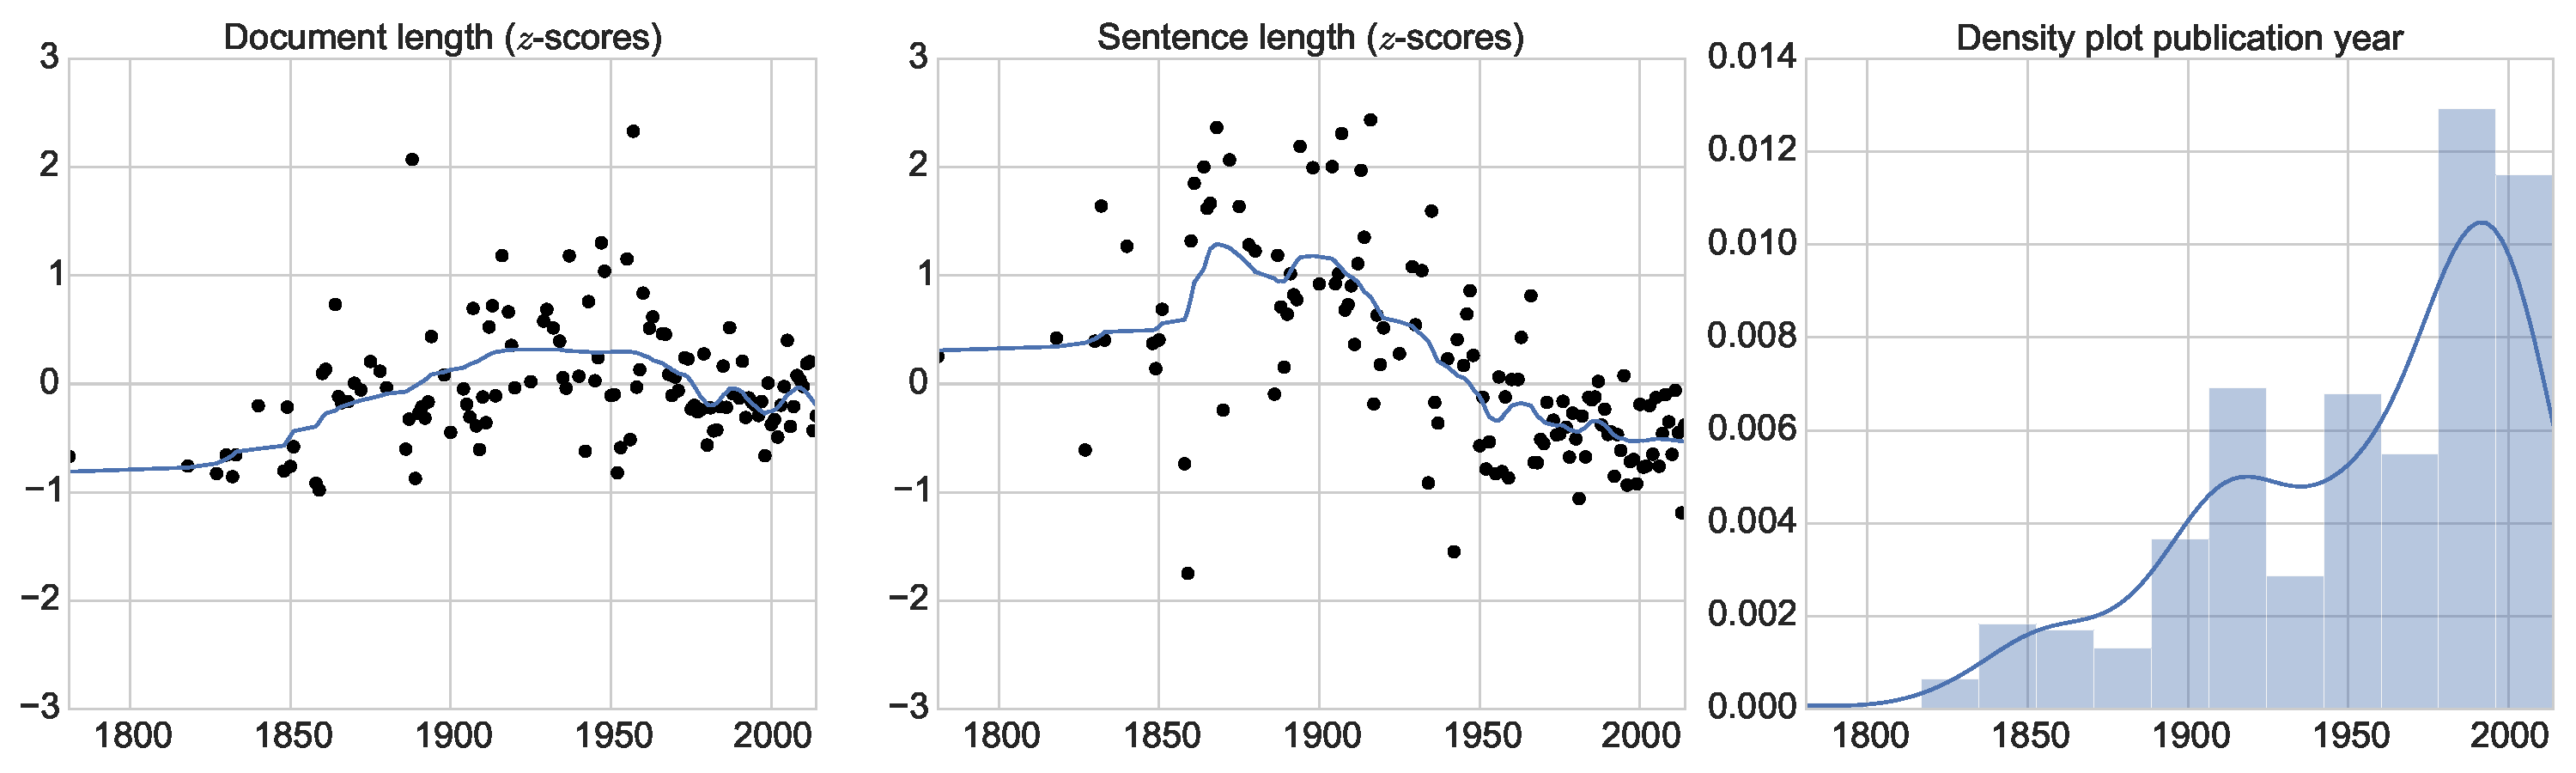
\includegraphics[width=\textwidth]{images/statistics}
\caption{Diachronic visualization of some general statistics about the ``Red Riding Hood'' corpus. The subplots (from left to right) in this figure visualize: the average $z$-scores of the document length per year (expressed in word forms), the average $z$-scores of the sentence length per year (expressed in word forms) and a kernel density plot of the year of publication of the stories.}
\label{fig:corpus-statistics}
\end{figure}

I constructed a tokenized version of the ``Red Riding Hood'' collection using the tokenizer Ucto.\footnote{See \url{https://languagemachines.github.io/ucto/} and corresponding manual \url{https://github.com/LanguageMachines/ucto/raw/master/docs/ucto_manual.pdf}.} The total number of words in the tokenized version amounts to 493,169 (including punctuation). In their lowercased form, 10,683 of these word forms occur uniquely. On average each year in the corpus ranging from 1781 to 2015 is represented by about 3 stories. Stories consist of 1155 word forms on average. Some of the general statistics of the corpus have been diachronically visualized in Figure \ref{fig:corpus-statistics}. The subplots (in order of appearance) in this figure visualize the average document length per year, the average sentence length per year and the number of retellings of ``Red Riding Hood'' published in a particular year. For reasons of comparability, I normalized the frequencies in the first two plots to their $z$-score. As can be observed from the density plot over the publication years of the stories, the corpus is rather skewed towards more recently published versions of ``Red Riding Hood''. This bias will be taken into account in the subsequent analyses. Looking at the first subplot, we can observe that the document length of the stories remains generally stable over time. When we inspect at the average sentence length, however, we note a steady decrease starting at the beginning of the \nth{20} century. We might hypothesize that this trend fits a development in which authors more and more adapt their retelling towards their young readers, who generally prefer shorter over longer sentences. However, more materials and research are required to assess whether the observed trend is representative of a development in children's literature at large. 

\subsection{Story Annotations}\label{sec:annotations}

Variation is one of the three preconditions described by Darwin for biological evolution. Without variation, there is nothing to be selected and hence no change can take place. Because of its central position to his theory, Darwin documents the variation he observed between members of the same species in great detail. An exemplary quote about variation about pigeons reads as follows:
\begin{quote}
    The proportional width of the gape of mouth, the proportional length of the eyelids, of the orifice of the nostrils, of the tongue (not always in strict correlation with the length of beak), the size of the crop and of the upper part of the oesophagus; the development and abortion of the oil-gland; the number of the primary wing and caudal feathers; the relative length of wing and tail to each other and to the body; the relative length of leg and of the feet; the number of scutellae on the toes, the development of skin between the toes, are all points of structure which are variable.\autocite[Darwin \emph{The Origin of Species}, cited in][27]{mesoudi:2011}
\end{quote}
\citeauthor{mesoudi:2011} argues that to justify the description of cultural change as a Darwinian evolutionary process, we must show that culture exhibits the same preconditions as biology\autocite[27--34]{mesoudi:2011}. An adaptation of Darwin's description of pigeon variation to ``Red Riding Hood'' could read as follows:
\begin{quote}
    The fabrics of Red Riding Hood's cap (cotton, silk, wool), the contents of her basket (is she carrying wine, bread, waffles, butter, juice, cake, lard), whether or not the girl meets with the wolf in the woods, the surroundings of grandmother's cottage (oaks, a hedge, a mill), whether the wolf eats granny and or Red Riding Hood and in what way (swallowing, gobbling, devouring, guzzling), whether the girl and her grandmother are saved and by whom (a woodcutter, a hunter, her father, animals in the forest), whether the wolf is killed and in what way (using an ax, a gunshot, a bat), whether the wolf's belly is filled with stones and who puts the stones in his belly, are all points of the story which are variable.
\end{quote}
Like Darwin, I could go on like this for several pages. If we look closely at all the different retellings of the story, the amount of variation is truly overwhelming. To establish a mapping of the variation, I subjected all 440 stories in the corpus to a questionnaire of more than 300 questions. The questionnaire consists of simple ``yes-no'' questions (e.g.\ \emph{Does the story explain the origin of Red Riding Hood's name?}), multiple choice questions (e.g.\ \emph{Where does Red Riding Hood encounter the wolf? (a) on the path, (b) away from the path, (c) somewhere else, (d) they don't meet}) and open questions (e.g.\ \emph{What is the lemma of the verb used to describe the wolf's eating of Red Riding Hood?}). Most questions in the questionnaire fit concepts from structural text analysis and narratology\autocite[E.g.][]{bal:2009,vanboven:2003}. The list of potential questions is virtually endless. I have attempted to compile a list of questions of which the answers constitute a detailed and rigorous text analysis. The questions can be classified under the following six categories: (i) genre, (ii) narration, (iii) space, (iv) motif, (v) time and (vi) character. 

\begin{figure}
    \centering
    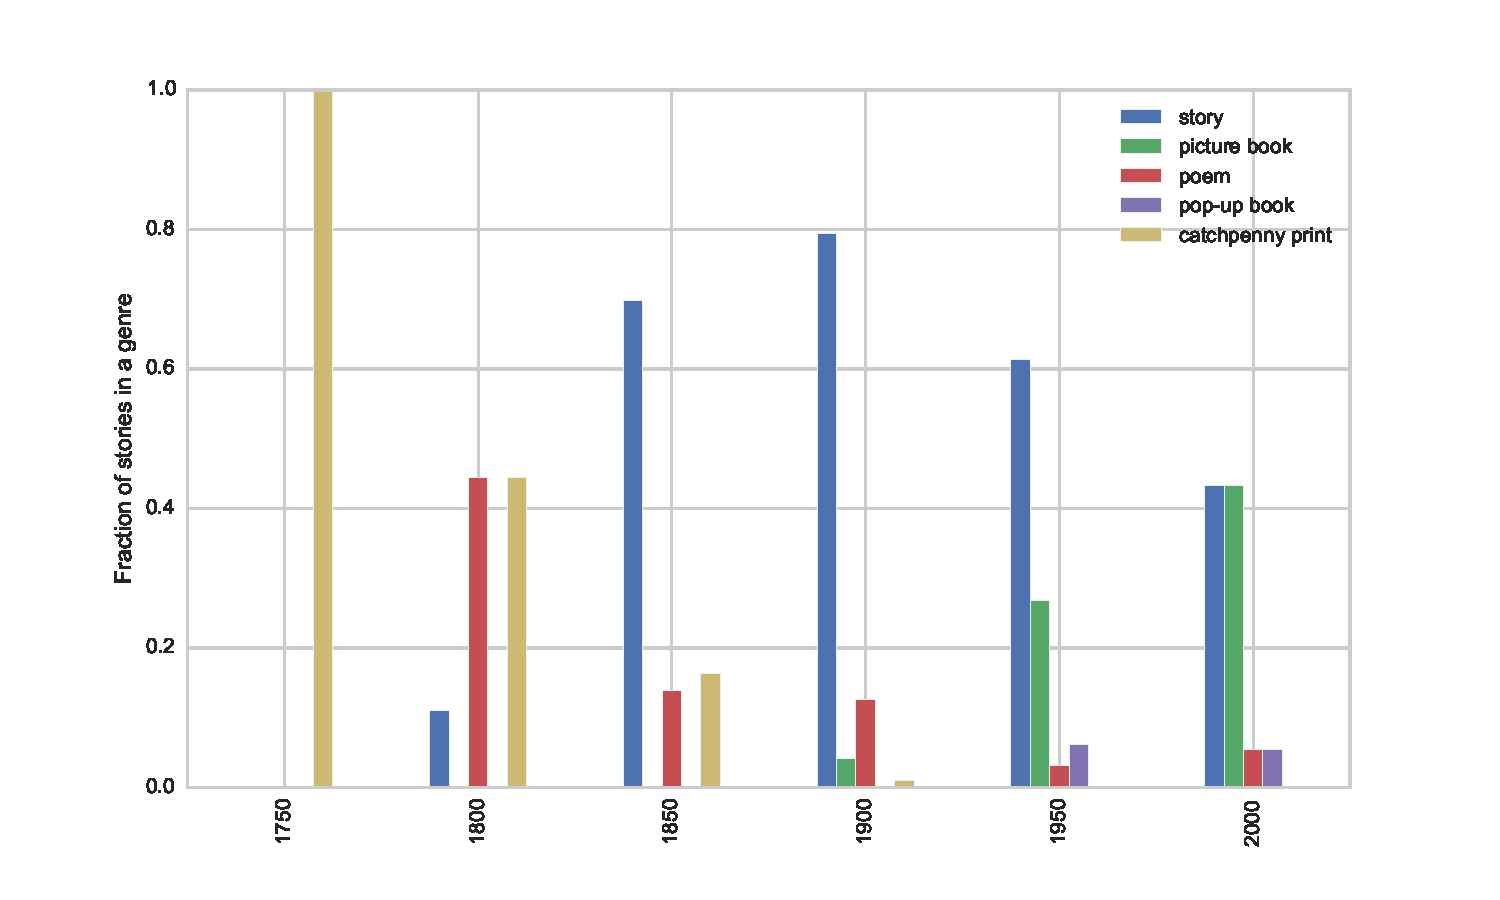
\includegraphics[width=\textwidth]{images/genre}
    \caption{Population plot of the five most frequently occurring genres in the ``Red Riding Hood'' collection. We calculate the fraction of stories published in a particular genre for every 50 years.}
    \label{fig:genre}
\end{figure}

\paragraph{(i) Genre} In the category `genre' we find questions designed to distinguish between kinds of stories in form and content. The collection of ``Red Riding Hood'' retellings contains the following genres: regular stories, picture books, pop-up books, theater, comics, puzzles, picture story, catchpenny prints and poems. A story with illustrations is not necessarily classified as a picture book. Only stories in which the pictures take central position with an accompanying text are considered to be picture books. As some stories belong to multiple genres, it was allowed to provide multiple answers. As can be observed from Figure \ref{fig:genre}, poems were a popular form for Dutch authors to tell the story in the second half of the \nth{19} century, whereas in more recent years, we discover a steady increase in the number of picture books. 

\paragraph{Narration (ii)} The second category of questions deals with the narration of the story. Most importantly, this category addresses the narrator of the story or -- in narratological terms -- the question of the speech-position from which the narrative contents of a story as a whole originates. Most versions of ``Red Riding Hood'' are classified as third-person narratives. In recent years retellers of ``Red Riding Hood'' have experimented with different forms of narration such as the first-person narrative. An interesting example of a first-person retelling is the one by the Dutch author Ivo de Wijs, which is part of the collection \emph{En ze leefden nog\ldots Sprookjes op Rijm}\autocite{wijs:2011}. The potentially hilarious effect of telling ``Red Riding Hood'' from a first person point of view becomes especially clear after Red Riding Hood is gobbled up by the wolf:

\vspace{\abovedisplayskip}
\begin{minipage}[c]{\textwidth}
\begin{Parallel}[c]{0.5\textwidth}{0.5\textwidth}
{\small
\ParallelLText{
\noindent
In de maag van het gulzige beest\\
Zat mijn oma, een tikkie bevreesd\\
Ze zei: `Meisje, je komt als geroepen\\
Want we moeten hier dadelijk uit\\
Stel je voor dat dat monster besluit\\
Ons gezamenlijk uit te gaan poepen'
}

\ParallelRText{
\noindent
In the tum of the devouring beast\\
Was my granny, a little afraid\\
She said: `Girl, you're just in time\\
Because we have to leave immediately\\
What if that the monster descides\\
to poop us out collectively'
}
}
\end{Parallel}
\end{minipage}

\vspace{\belowdisplayskip}
\paragraph{Space (iii)} The third category of questions deals with space. The questions aim to collect information about e.g.\ the location or the surroundings of grandmothers house. 

\paragraph{Motif (iv)} The largest group in the questionnaire is category four, which contains various questions about smaller and larger motifs, e.g.\ \emph{Is Red Riding Hood eaten by the wolf?}\ or \emph{Is the wolf's belly filled with stones or some other material?}. Category four also queries the main episodes of the story. Examples of questions are: \emph{Does the story contain a cautionary scene in which the mother of Red Riding Hood warns her about the dangers in the forest?} and \emph{Does the text describe a scene in which Red Riding Hood returns back home?} The Grimms' version of ``Red Riding Hood'' contains a rarely retold and virtually unknown second ending to the story. In this ending -- a kind of epilogue or sequel -- Red Riding Hood, barely recovered from her previous adventures, visits her grandmother again. In the woods she meets another wolf but this time she shows obedience and proves that she has learned her lesson. Together with her grandmother she manages to kill the wolf by making him fall from the roof into a big stone trough. The Dutch ``Red Riding Hood'' collection contains thirteen version in which this second episode is retold.

\paragraph{Time (v)} The category `time' contains questions that discuss the ordering of events, the passing of time and tension and irony. Examples of questions are: \emph{Does Red Riding Hood encounter the wolf before or after she strays from the path?} and \emph{If the wolf is killed, does that happen before or after Red Riding Hood (and her grandmother) are rescued?}. Questions about irony and tension were included in the category time, because they deal with expectations and anticipations of readers (e.g.\ `What will happen next?'). The climactic scene of the wolf in disguise can be read as an example of dramatic irony in which the girl naively believes the wolf to be her granny. To be able to understand this irony, children must have grown a `theory of mind', which allows them to reason about others in terms of goals and intentions. Theory of mind is one of the most important concepts in social-psychology and social evolution theory\autocite[see e.g.][]{tomasello:1999}, yet literary and folktale studies have only scantily paid attention to it\autocite[Cf.][]{boyd:2009}. In the development of a full-blown theory of mind, children learn about `beliefs' and `false beliefs'. In the context of ``Red Riding Hood'', this knowledge enables children to understand that the girl \emph{believes} that it is her grandmother lying in the bed, yet they know about the actual state of things and hence that this belief is false. Knowledge about (false) beliefs is of crucial importance in our life to make predictions about the behavior and intentions of others. ``No wonder,'' \citeauthor{boyd:2009} argues, ``that point of view and dramatic irony play such central roles in fiction, or that the gap between appearance and reality is such a wide-spread theme''\autocite[149]{boyd:2009}. Retellings of ``Red Riding Hood'' play with this theme. Sometimes authors explicitly anticipate the potential downer ending at the outset of the story, especially when there is no salvation scene. In other retellings, authors feel the need to make explicit that after being swallowed, the girl and her grandmother are still alive and well in the tummy of the wolf. Yet other versions omit the traditional switch of perspective from Red Riding Hood to the wolf and continue to keep track of the actions of the girl. In such versions, it is not yet clear to the reader who lies in the bed at the moment the girl arrives at her grandmother's cottage. This narrative strategy leads to a reading of the story without false belief and has a stronger effect of surprise. 

\paragraph{Character (vi)} Without the characters there would be no story. The last category contains questions about the participants in the stories. These include questions about the presence or absence of characters (e.g.\ \emph{Is Red Riding Hood's mother present in the story?}), about their physical properties (e.g.\ \emph{Does the story describe any physical properties of Red Riding Hood?}), about their clothing (e.g.\ \emph{Does the text make explicit reference to Red Riding Hood's hood?}), or about their personality traits (e.g.\ \emph{Is the wolf referred to as a ``(big) bad wolf''?}). 

\subsection{The Rise of the Big Bad Wolf}
In this section, I highlight one group of questions in some detail, viz.\ those dealing with the way characters are introduced to the story. Writers and storytellers have two basic introduction strategies to their disposal: They can introduce a character by means of (i) \emph{indefinite} reference (using an indefinite article, e.g.\ Dutch \emph{een}) or (ii) \emph{definite} reference (using a proper name or a definite article, e.g.\ Dutch \emph{de}).\autocite[See e.g.][]{deJong:1987,lyons:1999,radden:2007} Indefinite reference is generally used to introduce `new information', i.e.\ information the writer deems inaccessible to the reader. Definite reference, on the other hand, is typically used to refer to `given information' in which case the writer assumes that the reader is able to identify the intended referent. Folktale characters are typically introduced as `new' -- hence, their referent is introduced by means of an indefinite article at first mention, as in the following opening sentence from Perrault's \emph{Le petit Chaperon rouge}: ``Once upon a time there was \emph{a} little village girl\ldots'' Once introduced, the girl becomes given information, i.e.\ she becomes part of the set of referents that can be assumed to be accessible to the reader. This allows the writer to refer to the girl using definite reference in subsequent parts of the story. In the linguistic literature, the concept `discourse reference' is employed to indicate this transition from indefinite to definite reference, as it depends on the progression of discourse\autocite[98]{radden:2007}. Referents can also count as given information when they are (assumed to be) part of the shared socio-cultural world knowledge of a writer and a reader. This type of reference is called `unique reference'\autocite[99]{radden:2007}. Such entities can be referred to by means of definite reference even though they have not been introduced in the preceding discourse. 

I hypothesize that with the increasing familiarity of the story over time and its consequent entrenchment in culture\autocite[Cf.][]{beckett:2002}, the characters of ``Red Riding Hood'' become more and more part of the shared world knowledge of a writer and her or his audience. In other words, they become `given information'. Readers have expectations about the course of the story and appearance of certain characters, and writers assume their audience to know at least some version of the story. Indicative of their expectations, readers often act surprised when they discover that there is no rescuer in Perrault's version of the story. The entrenchment of the characters is exemplified by what \citeauthor{beckett:2002} calls fairy tale salads\autocite[Cf.\ chapter 7 in][]{beckett:2002}. These are stories in which characters from various popular fairy tales are transferred to new contexts without loosing their identity and accompanying literary and cultural expectations.

\begin{figure}
\centering
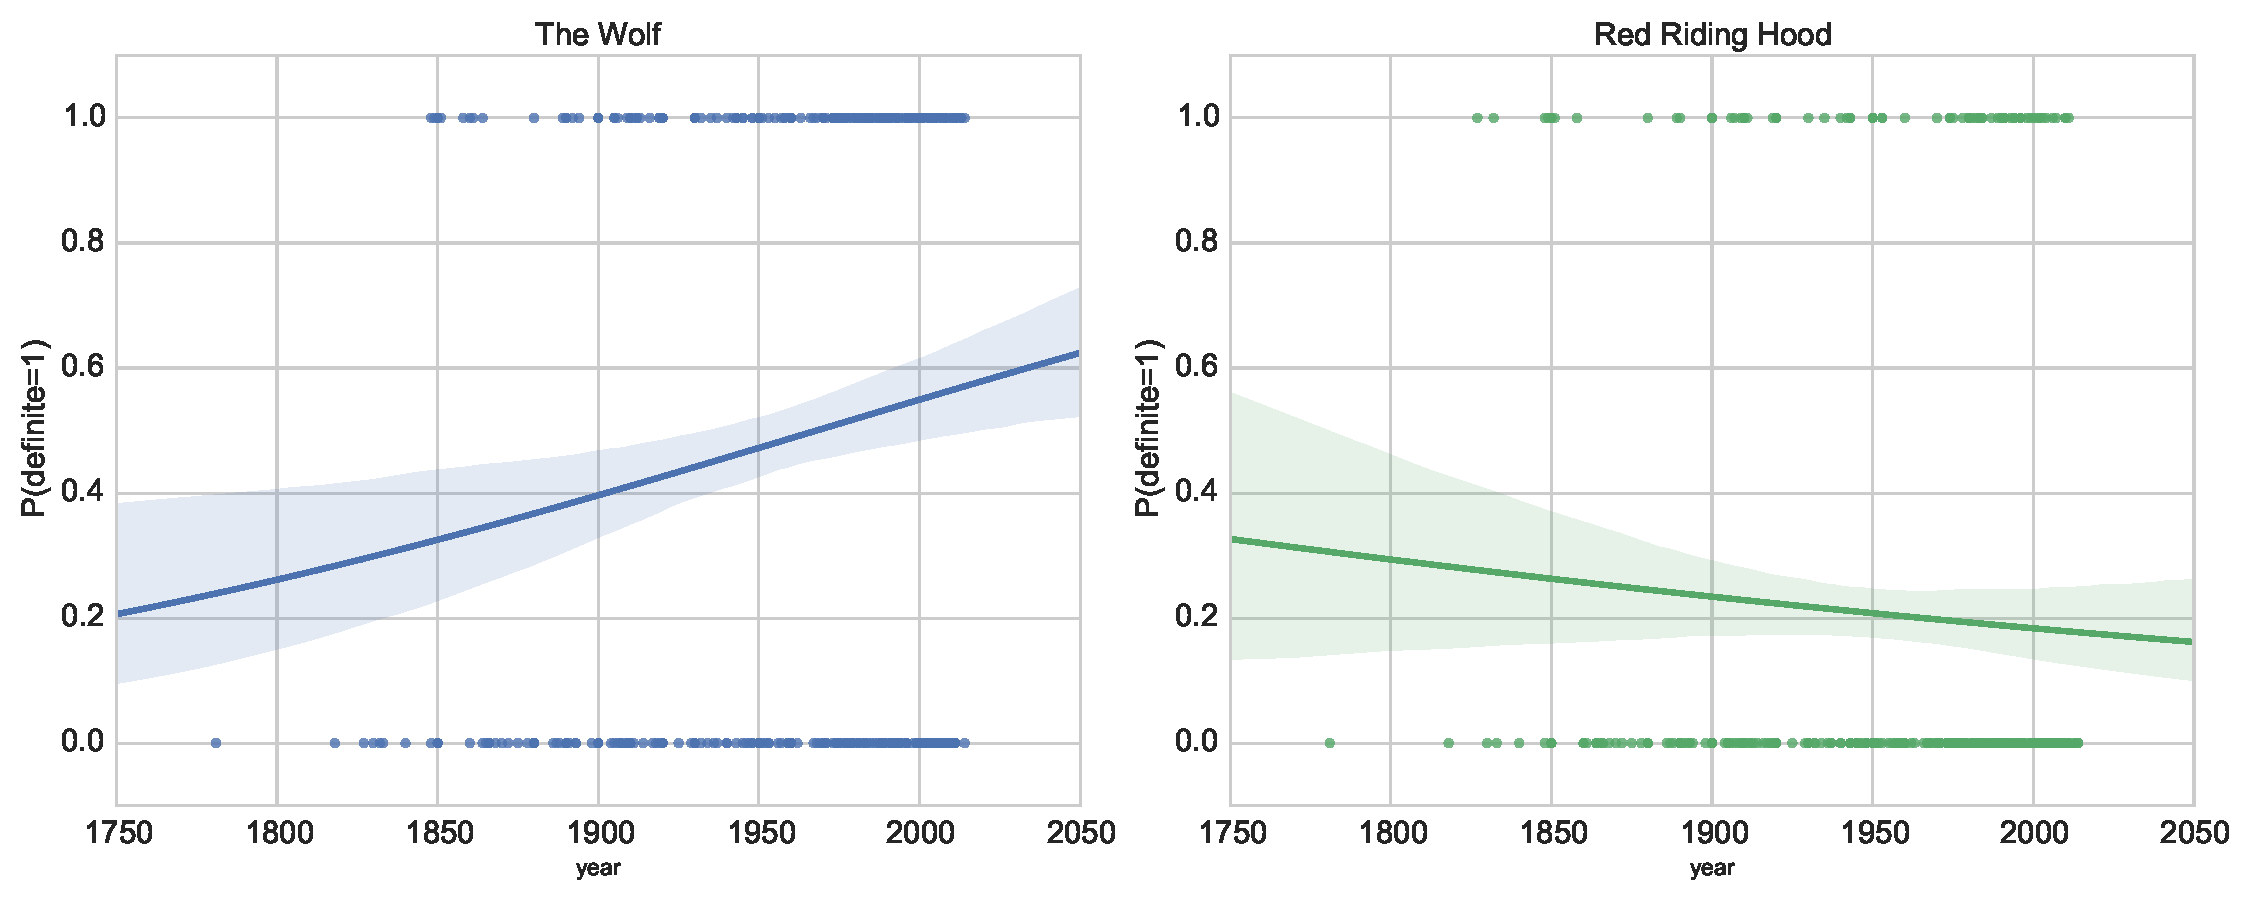
\includegraphics[width=\textwidth]{images/definite}
\caption{Plots showing definite (points with a value of 1.0) and indefinite references (points with a value of 0.0) used to introduce the wolf and Red Riding Hood in the corpus. The line represents the regression model fits to these points, the shade of which shows the confidence intervals.}
\label{fig:definite}
\end{figure}

If my hypothesis holds, we may expect an increase over time in the use of unique reference to introduce the characters of ``Red Riding Hood'' in favor of discourse reference. More specifically, I predict that the probability of introducing the characters by means of definite reference increases as a function of time. In the following analysis, I limit myself to the introduction of the two main characters: Red Riding Hood and the wolf. The question in the questionnaire corresponding to their introduction reads as follows: 
\begin{quotation}
\noindent\emph{Is Red Riding Hood / the wolf introduced to the story by means of definite or indefinite reference?} 
\end{quotation}
To test for the correlation between time and the increased use of unique reference, I subjected the answers given to these questions to two logistic regression analyses (i.e.\ one for Red Riding Hood and one for the wolf). The dependent variable in the regression is whether or not definite reference is used, and the predictor variable is the year of publication of a story. Figure \ref{fig:definite} displays the occurrences of definite and indefinite introductions for the wolf and Red Riding Hood. Points taking the value 1.0 represent introductions by means of definite reference; introductions with indefinite reference take the value 0.0. The curved line represents the fit of the regression model to the data. The shade reflects the confidence intervals of the fit. We can observe that the estimated probability for definite introductions of the wolf increases steadily over time. Analysis of the logistic regression model revealed that the effect of time is significant ($\beta=0.006, \textrm{SE} = 0.002, z = 2.887, p < 0.004$). For Red Riding Hood, by contrast, the plot shows a slight decrease in the estimated probability of definite introductions over time. This effect, however, is not significant ($\beta=-0.003, \textrm{SE}=0.002, z=-1.238, p > 0.2$).\footnote{The time laps in the collection might introduce a bias into the models. To account for this bias, I performed a logistic regression analysis in which the predictor variable `year' is replaced by a variable that increases by 1 with every subsequent year of publication in the corpus. The results of these analyses were similar to the previous ones, both for the wolf ($\beta=0.008, \textrm{SE} = 0.003, z = 2.634, p < 0.008$) and for Red Riding Hood ($\beta=-0.004, \textrm{SE} = 0.004, z = -1.132, p > 0.2$).}

How should we interpret the difference between the two model fits? I suggest that the probability of definite introductions of Red Riding Hood is generally low, because her introduction is constrained by the genre-specific opening sentences in which she is introduced (e.g.\ ``Once upon a time\ldots'' or ``In a country far, far away\ldots''). Because of their conventional nature, such opening phrases request the use of indefinite reference to introduce characters to a story\autocite[For a more general account of opening formulas in folktales, cf.][]{Karsdorp:2013tk}. Interestingly, in the ``Red Riding Hood'' collection these formulaic opening phrases have become even more conventional over time\footnote{The analysis of a logistic regression model shows a significant effect of time ($\beta=0.008, \textrm{SE} = 0.002, z = 3.733, p < 0.000$).}, thus making definite introductions even less likely. The wolf, on the other hand, is predominantly introduced after the cautionary scene, at which moment the constraints of conventional opening phrases no longer apply. The significant increase over time in the use of unique reference to introduce the wolf reflects the increasing familiarity of the story and the consequent expectations of readers about the appearance of certain characters. 

\subsection{Annotation Evaluation}
All stories in the collection have been subjected to the questionnaire. Using a self-developed annotation application\footnote{See \url{http://github.com/fbkarsdorp/roodkapje}.}, I annotated the complete collection. To assess the reliability of the annotations, a second annotator filled in the questionnaire for ten percent of the collection, after which discrepancies with my own annotations were discussed. The amount of agreement between the annotators was measured by means of the $F1$-score.\footnote{Cohen's $\kappa$-statistic \citeyear{cohen:1960} is not suitable for this evaluation, because it is impossible to compute the number of true negatives for certain open questions in the questionnaire.} The results showed strong agreement between the annotations ($F1 = 0.95$). All categorical variables (resulting from multiple choice and open questions) where converted into binary indicator variables. The resulting $m \times n$ matrix $S$ consisted of $m=440$ stories, each of which was represented by $n=2444$ binary variables.

\section{Methods}\label{sec:methods}

\subsection{Distance Measures}
Recall from the introduction that the goal is to identify a set of potential pre-texts for each story in the ``Red Riding Hood'' collection. In this study, I make the simplifying assumption that stories that are more similar to a particular story in terms of their annotations are more likely to have formed their pre-text than other stories. The distance (or similarity) between two stories can be assessed by means of a distance measure, which summarizes the distance between two stories in terms of a pairwise comparison of the answers given to each of the questions in the questionnaire. Importantly, the choice for a particular distance measure can have a severe impact on what is considered to be similar and what is not\autocite[Numerous papers have been published in which various binary distance metrics and similarity coefficients have been proposed. For an in-depth comparison, cf.][]{choi:2010}. 

We can distinguish two main groups of binary distance measures: `negative match \emph{inclusive}' and `negative match \emph{exclusive}' measures. Negative match inclusive measures assume that the absence of two features contributes to the similarity between two objects. In the context of story annotations, this implies that the absence of, for example, the rescue scene in two particular stories adds to the similarity between them. Negative match exclusive measures do not include negative matches in their similarity estimation, and thus do not account for the absence of the rescue scene. The potential downside of negative match inclusive measures becomes especially clear in the context of low frequency features. Take the contents of Red Riding Hood's basket as an example. In only three versions in the collection, Red Riding Hood brings a bottle of milk to her grandmother. Negative match inclusive measures reinforce the similarities between all stories in which the milk is \emph{absent}. Negative match exclusive measures, by contrast, will only reward the similarities between these three versions. More generally, the chance that two stories invoke a negative answer increases as questions become more specific. This does not, however, necessarily imply that the two stories are more similar. 

\begin{figure}
\centering
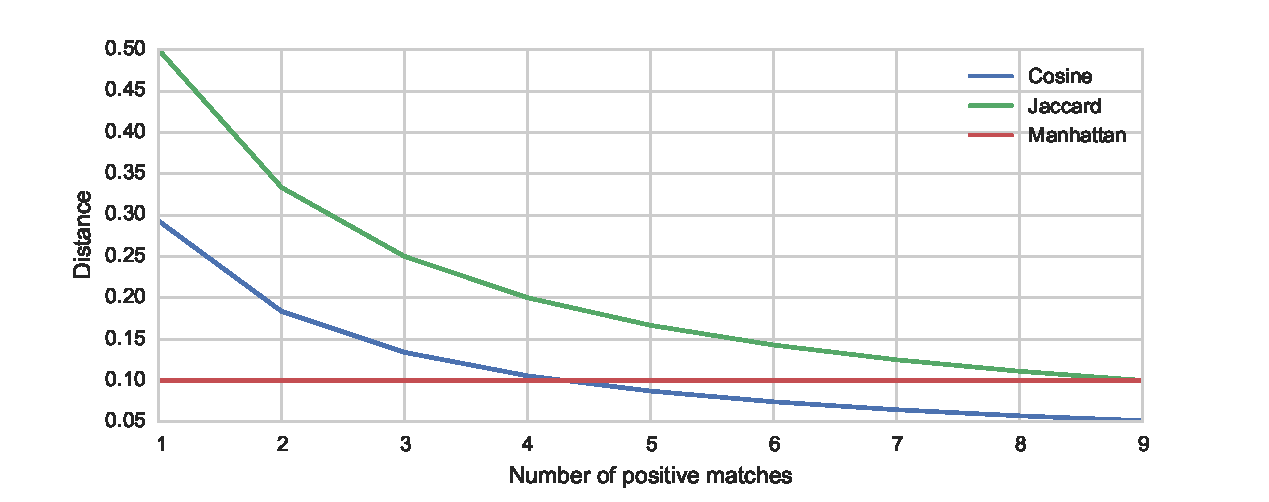
\includegraphics[width=\textwidth]{images/mismatches}
\caption{Plot showing the differences between the Manhattan distance, Jaccard dissimilarity index and Cosine distance for pairs of vectors with an increasing number of positive matches while keeping the number of mismatches constant at 1. The size of the vectors is 10.}
\label{fig:mismatches}
\end{figure}

In the subsequent analyses, I will compare three binary distance measures: (i) Manhattan distance, (ii) Jaccard dissimilarity index, and (iii) Cosine distance. All three measures have their own assumptions about what is to be considered similar or distant. In what follows, I provide a detailed description of these measures, with which I hope to clarify some of these assumptions.\footnote{For this description I adopt the terminology used by \autocite{choi:2010}.} Let $a$ represent the number of questions to which two stories $i$ and $j$ provide a positive answer. Let $b$ be the number of questions that are positively answered by story $i$ and negatively by story $j$. Finally, let $c$ represent the number of questions negatively answered by story $i$ and positively by story $j$. The sum of $b$ and $c$ represents the total number of mismatches between two stories and is equivalent to the Manhattan distance (also known as the city block distance or $\ell_1$ norm):
\begin{equation}
d_1 = b + c
\end{equation}
The Manhattan distance is an example of a negative match inclusive measure and is based on the assumption that only mismatches contribute to the distance between two stories, and conversely that positive matches and negative matches add to their similarity. 

The Jaccard similarity index is an example of a negative match exclusive measure. It is computed as the number of positive matches ($a$) divided by the sum of positive matches and mismatches ($a + b + c$). In set based terms, it computes the fraction of the length of the intersection between two stories over the size of their union. The complement of this fraction represents the dissimilarity between two stories:
\begin{equation}
d_J = 1 - \frac{a}{a + b + c}
\end{equation}
The Cosine distance is an example of a negative match exclusive measure as well. It is computed as follows:
\begin{equation}
d_C = 1 - \frac{a}{\sqrt{(a + b) \times (a + c)}}
\end{equation}
To get an impression of the effect of each of these distance measures, consider the following four binary vectors, each representing one story: 
\begin{align*}
\mathbf{a}^{(1)} & = \begin{bmatrix*} \dnum{0} & \dnum{1} & \dnum{0} & \dnum{1} & \dnum{0} & \dnum{0} \end{bmatrix*} \\
\mathbf{a}^{(2)} & = \begin{bmatrix*} \dnum{0} & \dnum{1} & \dnum{0} & \dnum{1} & \dnum{0} & \dnum{1} \end{bmatrix*} \\
\mathbf{a}^{(3)} & = \begin{bmatrix*} \dnum{1} & \dnum{1} & \dnum{1} & \dnum{1} & \dnum{1} & \dnum{1} \end{bmatrix*} \\
\mathbf{a}^{(4)} & = \begin{bmatrix*} \dnum{1} & \dnum{0} & \dnum{1} & \dnum{1} & \dnum{1} & \dnum{1} \end{bmatrix*}
\end{align*}
The Manhattan distance $d_1(\mathbf{a}^{(1)}, \mathbf{a}^{(2)}) = d_1(\mathbf{a}^{(3)}, \mathbf{a}^{(4)}) = 1$, because the two pairs contain an equal number of mismatches. The Jaccard dissimilarity index does not consider the negative matches and thus returns a distance of approximately 0.33 between $\mathbf{a}^{(1)}$ and $\mathbf{a}^{(2)}$ and 0.16 between $\mathbf{a}^{(3)}$ and $\mathbf{a}^{(4)}$. As expected, the Cosine distance between $\mathbf{a}^{(1)}$ and $\mathbf{a}^{(2)}$ (0.18) is also larger than between $\mathbf{a}^{(3)}$ and $\mathbf{a}^{(4)}$ (0.08). The magnitude of the difference, however, is larger for the Jaccard dissimilarity index than for the Cosine distance. This effect can also be observed from Figure \ref{fig:mismatches}, which shows the differences between the three distance measures for pairs of vectors with an increasing number of positive matches, while keeping the number of mismatches constant at 1.

\subsection{Time Span Normalization}
The goal is to produce a ranking of texts for each story in the collection, in which the top items represent the most likely pre-texts. Using one of the above-mentioned distance measures, we can compute the distance between a story $i$ published in year $t_i$ and all potential pre-texts. The set of potential pre-texts for story $i$ is defined as all stories published in or before year $t_i$, i.e.\ $\{j | \forall j \in \{1, 2, \ldots, m\} \wedge t_j \leq t_i \wedge i \neq j\}$. To produce a final ranking, the pre-texts are sorted according to their distance to $i$ in ascending order. 

Given a ranking of potential pre-texts, we can evaluate the timespan between a particular retelling and its $k$ most likely pre-texts. Simply taking the difference between year $t_i$ and $t_j$, however, does not suffice, because older stories have a smaller set of potential pre-texts than stories published in later years, and this potentially introduces a bias in the results towards shorter timespans. Since the oldest story in the collection stems from 1781, the maximum timespan for a story published in, for example, 1850 is only 69 years, whereas for stories published in the \nth{21} century, the maximum timespan is more than 200 years. To account for this bias, I propose the following equation, which normalizes the time differences with respect to the total timespan of the collection:
\begin{equation}
\Delta t_{ij} = | t_i - t_j | \frac{t_{\max} - t_{\min}}{t_i - t_{\min}},
\label{eq:timepenalty}
\end{equation}
where $t_i$ and $t_j$ refer to the year of publication of story $i$ and $j$ respectively. $t_{\min}$ and $t_{\max}$ correspond to the publication years of the oldest and youngest story in the collection. Figure \ref{fig:time-penalty} illustrates the effect of applying the normalization. In this plot, four hypothetical stories published in the years 1850, 1900, 1950 and 2000 each select a story from 1800 as their most likely pre-text. Without the normalization method, the time differences between the stories and this pre-text will be 50, 100, 150 and 200 years respectively. As can be observed from the plot, the normalization method adjusts all time differences to 200 years.

\begin{figure}
\centering
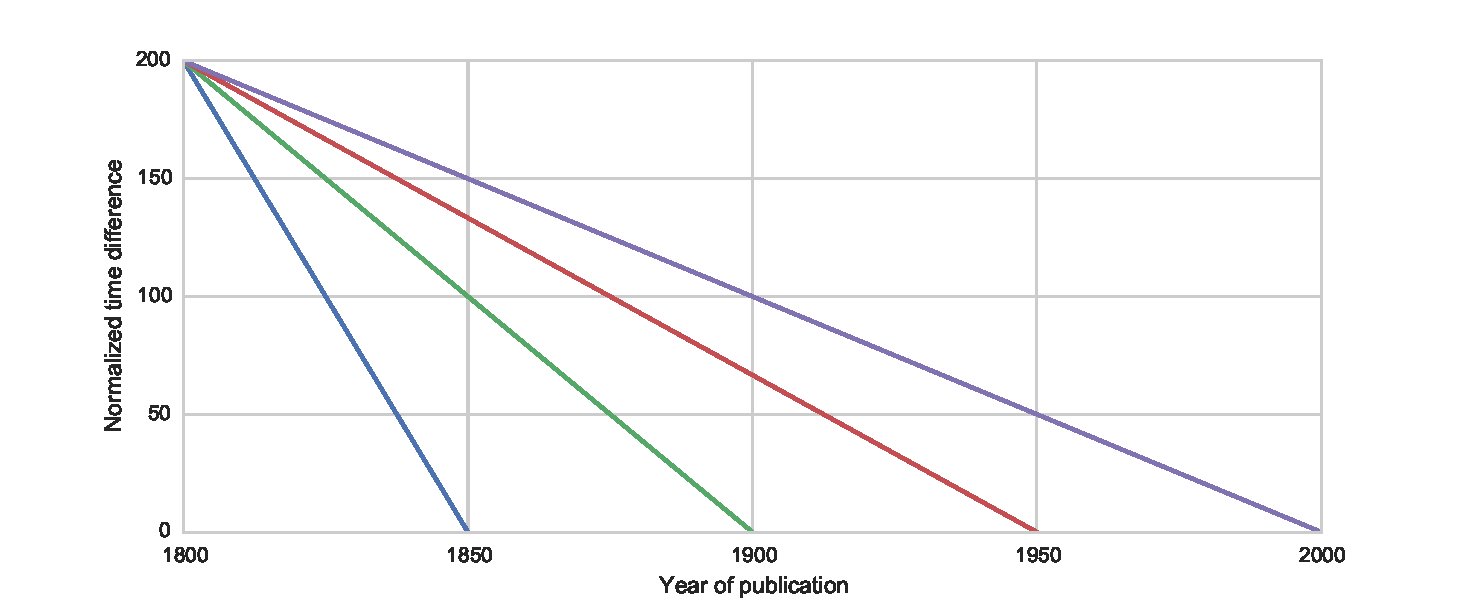
\includegraphics[width=\textwidth]{images/timepenalty}
\caption{Visual illustration of the time difference normalization method, cf.\ Eq.~\ref{eq:timepenalty}.}
\label{fig:time-penalty}
\end{figure}

\subsection{Reliability Assessment}
The performance of the proposed methodology to rank pre-texts depends on a number of factors. We have already seen that the choice for a particular distance measure can have a strong effect on the final rankings. The number of variables and the selection of particular variables can have a similar impact on the results. The dependence on all these factors brings the reliability of the results into question. In what follows, I propose two ways to assess the reliability of the analyses.

As a first way to assess the consistency of the results, I perform a bootstrap analysis. The general idea behind this analysis is to approach the data from various angles for a large number of trials. In each trial we randomly select (with replacement) 10\% of the features from the complete feature space. Using these randomly chosen features, a ranking of $k$ most likely pre-texts can be established for each story in the collection. Each trial potentially returns different results. The final results are obtained by applying a majority voting mechanism, which selects those results that have reached mode consensus over all trials. In the analyses I will present below, the bootstrap analysis was set to run for 5000 trials\autocite[For more information about the bootstrap procedure, see][]{good:2006}.

As a second reliability assessment, I compare the results to those obtained by using a different feature representation. I choose to employ a bag-of-words model, which represent documents as histograms over the vocabulary, i.e.\ as vectors of occurrence counts of words. For a document $d$ with a vocabulary size $V$ the vector representation $\mathbf{w}^{(d)}$ is given by $(w_1, w_2, \ldots, w_V)$, where $w_i$ represents the occurrence count of word $i$ in $d$. These representations can be used to compute the distance between two documents, e.g.\ by means of the Cosine distance. A clear advantage of bag-of-word models is the obviation of manual annotations for low-level features, such as lexical features. This comes with a price, however, because the many dimensions of word vector spaces may obfuscate the interpretability of the results. Another disadvantage of bag-of-words, at least for the purposes of the present study, is their sensitivity to spelling differences. The ``Red Riding Hood'' collection contains retellings written according to spelling conventions at various points in history. As a result, the rankings of pre-texts on the basis of bag-of-words models might reflect these spelling reforms, whereas we are more interested in rankings based on the actual contents of the stories. Despite this potential bias, I believe that bag-of-words models function as a useful background check to assess the reliability of the results obtained through ranking pre-texts on the basis of the answers given to the questionnaire (cf.\ Section \ref{sec:annotations}). 

I weigh the word frequency vector spaces by means of the well-known `term frequency-inverse document frequency' (tf-idf) weighting scheme\autocite{manning:2008}. This model weighs the occurrence counts of words in a document (tf) against the background of how many documents in the corpus contain those words (idf). The tf-idf transformed vector spaces put more weight on words with high term frequencies (i.e.\ words occurring often in a particular document) and relatively low document frequencies. Words with high tf-idf weights can be considered to be topical words, whereas words with low weights occur either too often (e.g.\ function words) or too infrequently (e.g.\ spelling mistakes) to be of topical value. In the experiments below, I compute the distance between stories by means of the Cosine distance. Again, I apply a bootstrap procedure in which for 5000 trials, I sample 10\% of the vector space to produce a ranking of potential pre-texts for each story in the collection.

\section{Results}\label{sec:results}

Table \ref{tab:result-statistics} presents the results of the analyses. For both feature representations (i.e.\ the questionnaire and the bag-of-words vectors) the table lists the mean ($\mu$), median ($\hat{x}$), and standard deviation ($\sigma$) of the timespan between stories and their most likely pre-text. In addition, the table shows the results obtained from applying the bootstrap procedure to each of these two feature representations. The bootstrap procedure produced slightly smaller numbers for both feature representations. Since these bootstrapped numbers represent the mode consensus computed by approaching the data from various angles over a large number of trials, they are to be considered to be the most reliable results. The three distance measures (Manhattan distance ($d_1$), Jaccard dissimilarity index ($d_J$), and Cosine distance ($d_C$)) generated nearly equivalent numbers, which is an indication of the robustness of the results. On average, the adjusted timespan between a retelling and its pre-text is about 30 years. However, as will be discussed in more detail below, the timespans distributions are rather skewed. Therefore, rather than using the mean $\mu$, it is more appropriate to use the median $\hat{x}$ as a measure of location, which amounts to approximately 17 years. This number for the bootstrapped bag-of-words model is about five years less, which indicates that, solely on the basis of their vocabulary, stories seem to select pre-texts in slightly closer temporal proximity. However, without further research, we cannot rule out the possibility that this difference is a reflection of spelling reforms and variation. 

It should be noted that the numbers listed in Table \ref{tab:result-statistics} do not conclusively resolve the question whether retellings are based on intermediate retellings and whether the development of ``Red Riding Hood'' in the Netherlands can be described as a process of `gradual accumulation of modification' (cf.\ Section \ref{sec:introduction}). There is no `ground truth' indicating which text formed the pre-text of a particular retelling, either because we cannot definitely retrieve it or because it is doubtful whether this concept of a ground truth is applicable to the idea of a pre-text at all. Thus, all we have at our disposal to investigate relations between stories is statistical distributions of timespans. The challenge, then, is to reject alternative hypotheses about the origins of these distributions.

\begin{table}
\centering
\begin{tabular}{llll}
\toprule
model                     & $d_1$                  & $d_J$                 & $d_C$                 \\ \midrule
                          & $\mu$ / $\hat{x}$  / $\sigma$  & $\mu$ / $\hat{x}$  / $\sigma$ & $\mu$ / $\hat{x}$ / $\sigma$ \\ \cmidrule(r){2-4}
questionnaire             & 35    / 21 / 38        & 33    / 18 / 38       & 33    / 18 / 38       \\
questionnaire (bootstr.) & 31    / 18 / 33        & 30    / 17 / 32       & 30    / 17 / 32       \\
bag-of-words              & --                     & --                    & 21    / 14 / 23       \\
bag-of-words (bootstr.)  & --                     & --                    & 18    / 12 / 20       \\
\bottomrule
\end{tabular}
\caption{Rounded mean ($\mu$), median ($\hat{x}$) and standard deviation ($\sigma$) of timespans adjusted according to Eq.\ \ref{eq:timepenalty}. Results are given for the questionnaire with the complete feature space, the bootstrap model applied to the questionnaire, the bag-of-words model and the bootstrap model applied to the bag-of-words model. The table shows results obtained by the Manhattan distance ($d_1$), Jaccard dissimilarity index ($d_J$) and the Cosine distance ($d_C$).}
\label{tab:result-statistics}
\end{table}

The first hypothesis is that the reported median timespans express artifacts of the data collection or the specific methods employed. Recall from Section \ref{sec:data} that the distribution of publications is rather skewed towards more recent publication years, and, as such, older retellings have a smaller pool of potential pre-texts to sample from than more recent retellings. More specifically, one might argue that the timespan distribution computed on the basis of the similarities between retellings and their pre-texts is not significantly different from a distribution in which pre-texts have been selected without any textual information, but, for example, on the basis of a uniform prior over previous generations. In such a distribution, a pre-text stems just as likely from the immediate previous year as from $n$ years back in time. To estimate such a distribution, I randomly select a year of publication for each story in the collection from the range $[t_{\min}, t_i]$, where $t_i$ is the year of publication of a story $i$ and $t_{\min}$ is the publication year of the first story in the collection (i.e.\ 1781). 

\begin{figure}
\centering
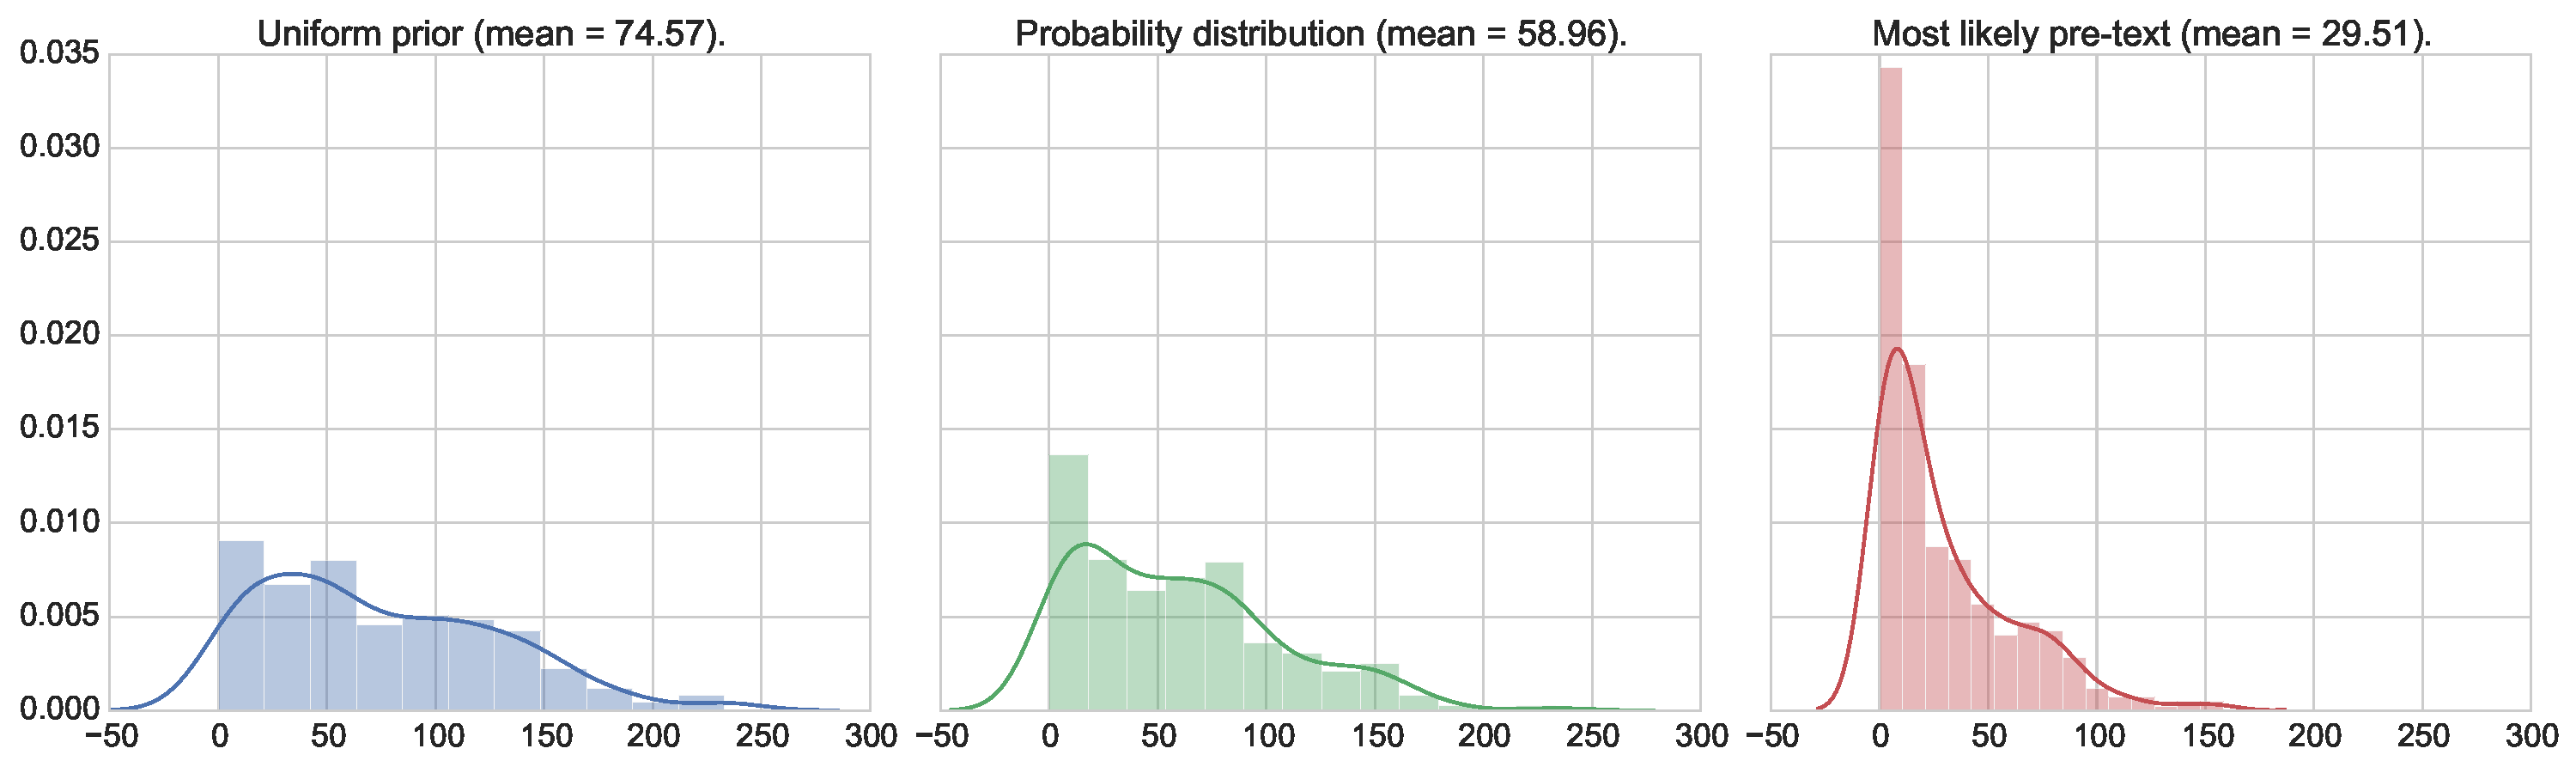
\includegraphics[width=\textwidth]{images/distributions}
\caption{Kernel density plots of timespan distributions. The left plot is generated using a uniform prior over previous generations. The plot in the middle represents a non-uniform random sample from the probability distribution over years of publication. The third plot presents the distribution over timespans that was estimated using the bootstrap procedure with $k=1$ and the Cosine distance $d_C$.}
\label{fig:timespan-distribution}
\end{figure}

Of course, a uniform prior over previous years of publications might be too naive and too easily rejected. I therefore test a second competing hypothesis, which investigates whether the extracted timespan distribution is significantly different from a distribution in which pre-texts are selected on the basis of a probability distribution over the observed years of publication in the collection. In this distribution, years in which many stories have been published have a higher probability than years in which only a few stories were attested. As such, this hypothesis more directly addresses the potential bias towards shorter timespans between stories and pre-texts resulting from the skewed distribution of publication years in the collection. To estimate this distribution of timespans, I randomly select a year of publication from the range $[t_{\min}, t_i]$ for each story $i$ in the collection on the basis of the probabilities associated with each publication year in the collection. 

Figure \ref{fig:timespan-distribution} presents the kernel density plots of the three timespan distributions. The right subplot displays the estimated text-based timespan distribution (computed using the bootstrap procedure and the Cosine distance). The left subplot displays the density of a random sample generated from a uniform prior over previous years of publication. A two-sample Kolmogorov-Smirnov test rejects the hypothesis that these two samples are drawn from the same distribution ($D=0.404, p < 0.0001$). This is confirmed by a Wilcoxon rank-sum test: $z=12.902, p < 0.0001$. The subplot in the middle represents a random sample generated on the basis of the probability distribution over years of publication in the collection. We can also safely reject the hypothesis that this sample is the same as the text-based timespan distribution (Kolmogorov-Smirnov test: $D=0.312, p < 0.0001$; Wilcoxon rank-sum test: $z=9.643, p < 0.0001$). 

Note that the subplots in Figure \ref{fig:timespan-distribution} display an increasingly skewed timespan distribution with pre-texts being published in temporal proximity of retellings. In what follows, I will formally characterize this skewed distribution. The Gamma distribution covers a wide range of skewness, and, as such, it appears to be a good candidate to fit the text-based timespan distribution. The probability density function of the Gamma distribution is given by: 
\begin{equation}
f(x; \alpha, \beta) = \frac{\beta^{\alpha} x^{\alpha-1} e^{-x \beta}}{\Gamma(\alpha)}
\end{equation}
for $x \ge 0$, and $\alpha,\beta > 0$. The shape parameter is represented by $\alpha$, and $\beta$ is the scale parameter. I perform a maximum likelihood estimation of the distribution parameters $\alpha$ and $\beta$. The parameters resulting in the smallest sum of square errors between the text-based distribution and the fitted distribution are given by $\alpha=0.84$ and $\beta=22.7$. To statistically assess the similarity between the fitted distribution and the text-based timespan distribution, I subject the two distributions to a two-sample Kolmogorov-Smirnov test and a Wilcoxon rank-sum test. Both statistical assessments yield non-significant results at the five percent level ($D=0.3, p > 0.1$ and $z = 1.257, p > 0.2$). Therefore, we cannot reject the null hypothesis that the distributions are the same, and hence, the text-based timespan distribution can be considered to be Gamma-distributed. Table \ref{tab:gamma-statistics} presents the results for the same analysis on four consecutive time periods. With the exception of the Kolmogorov-Smirnov test for the period 1850 -- 1900, no test is significant at the five percent level. This suggests that the Gamma distribution is applicable to the complete collection.

\begin{table}
\centering
\begin{tabular}{lllll}
\toprule
             & \multicolumn{2}{c}{Kolmogorov-Smirnov} & \multicolumn{2}{c}{Wilcoxon rank-sum} \\ \midrule
             & $KS$ & $p$         & $z$   & $p$         \\ \cmidrule(r){2-5}
1850 -- 1900 & 0.55 & < 0.004 & 1.677 & > 0.09  \\
1900 -- 1950 & 0.3  & > 0.2   & 0.703 & > 0.4   \\
1950 -- 2000 & 0.25 & > 0.4   & 0.839 & > 0.4   \\
2000 -- 2015 & 0.4  & > 0.05  & 0.947 & > 0.3   \\      
\bottomrule
\end{tabular}
\caption{Kolmogorov-Smirnov tests and Wilcoxon rank-sum tests for the null hypothesis that the text-based timespan distributions in four consecutive time periods are gamma-distributed.}
\label{tab:gamma-statistics} 
\end{table}

\section{Discussion}\label{sec:discussion}

The results presented in this article strongly suggest that retellings of ``Red Riding Hood'' are most similar to intermediate retellings. First, I have shown that such `intermediate retellings' can be refined as retellings that are published in close temporal proximity. Acknowledging that there is no definite way to ascertain that a particular author based her or his retelling on one specific pre-text~\autocite{stephens_mccallum}, I suggest that the focus should be shifted to textual resonances~\autocite[Cf.][]{frank:2010}, which form a stream of previous retellings. It was shown that this stream gradually changes in a cumulative way, with retellings modifying and adapting other retellings. As such, the transmission process of literary versions of ``Red Riding Hood'' in the Netherlands can be considered a cultural evolutionary process: in producing a new retelling, authors select from a variety of competing existing retellings and potentially introduce innovations, which can eventually replace existing story elements. If these innovations are, in their turn, adopted in further retellings, the cycle of variation-competition-inheritance leads to a gradual accumulation of modifications. Further examining the selection biases, this study indicates that retellings of ``Red Riding Hood'' are evidently not `second generation' stories that are simply based on one of the `classic' versions written by either Perrault or the Brothers Grimm, and it is also unlikely that retellers sample their base material from a uniform distribution over all previous generations. Instead, it appears that more recent versions, at a median of about 17 years, are more likely to inspire retellings than versions from older dates. 

Thus, the present study shows that age-dependent selection criteria can -- at least partially -- explain the differential fitness among competing retellings of ``Red Riding Hood''. Given this insight, we might wonder what this tells us about the development in children's literature at large and even cultural change in general. A key virtue of the cultural evolutionary approach as advocated in the present study is the use of idealized explanatory models of cultural change~\autocite[Cf.\ e.g.][]{mesoudi:2011,boyd_richerson:2005,lewens:2015}. Such models are deliberately kept simple in order to facilitate isolating and manipulating single variables under highly controlled conditions~\autocite{mesoudi:2011}. Yet, despite their simplicity, these models appear to have great informative strength in that they are able to explain unanticipated, complex population-level effects resulting from the actions of individuals~\autocite{mcelreath2005,lewens:2015}. The value of the current study lies in the fact that it considers the evolution of a cultural artifact using a particular methodology that can easily be compared to more parsimonious explanatory models of cultural change, and as such allows us to assess the explanatory strength of a model involving age-dependent selection. 

In recent years, several publications within the field of cultural evolution have shown that various population-level effects can in fact often be explained by means of an unbiased process in a neutral model of selection~\autocite[See e.g.][]{Bentley:2004,Mesoudi:2009}. This neutral model offers a parsimonious explanation for cultural change as it merely assumes individuals either copy the behavior from a randomly selected individual from the previous generation or they innovate and introduce a new cultural trait into the population. Whether or not individuals introduce an innovation is controlled by an innovation rate parameter $\mu$. With smaller values of $\mu$ the probability of innovation decreases. It has been shown that this simple model provides accurate predictions for a variety of cultural changes, such as the choice of baby names~\autocite{Hahn:2003}, the selection of keyword in academic publications~\autocite{Bentley:2008} and the popularity of dog breeds~\autocite{herzog:2004}. In fact, this random copying model, equivalent to biological genetic drift, appears to be so powerful that researchers in the cultural evolution research program consider it to be the null-hypothesis in the description of cultural evolutionary processes. 

\begin{sidewaysfigure}
\centering
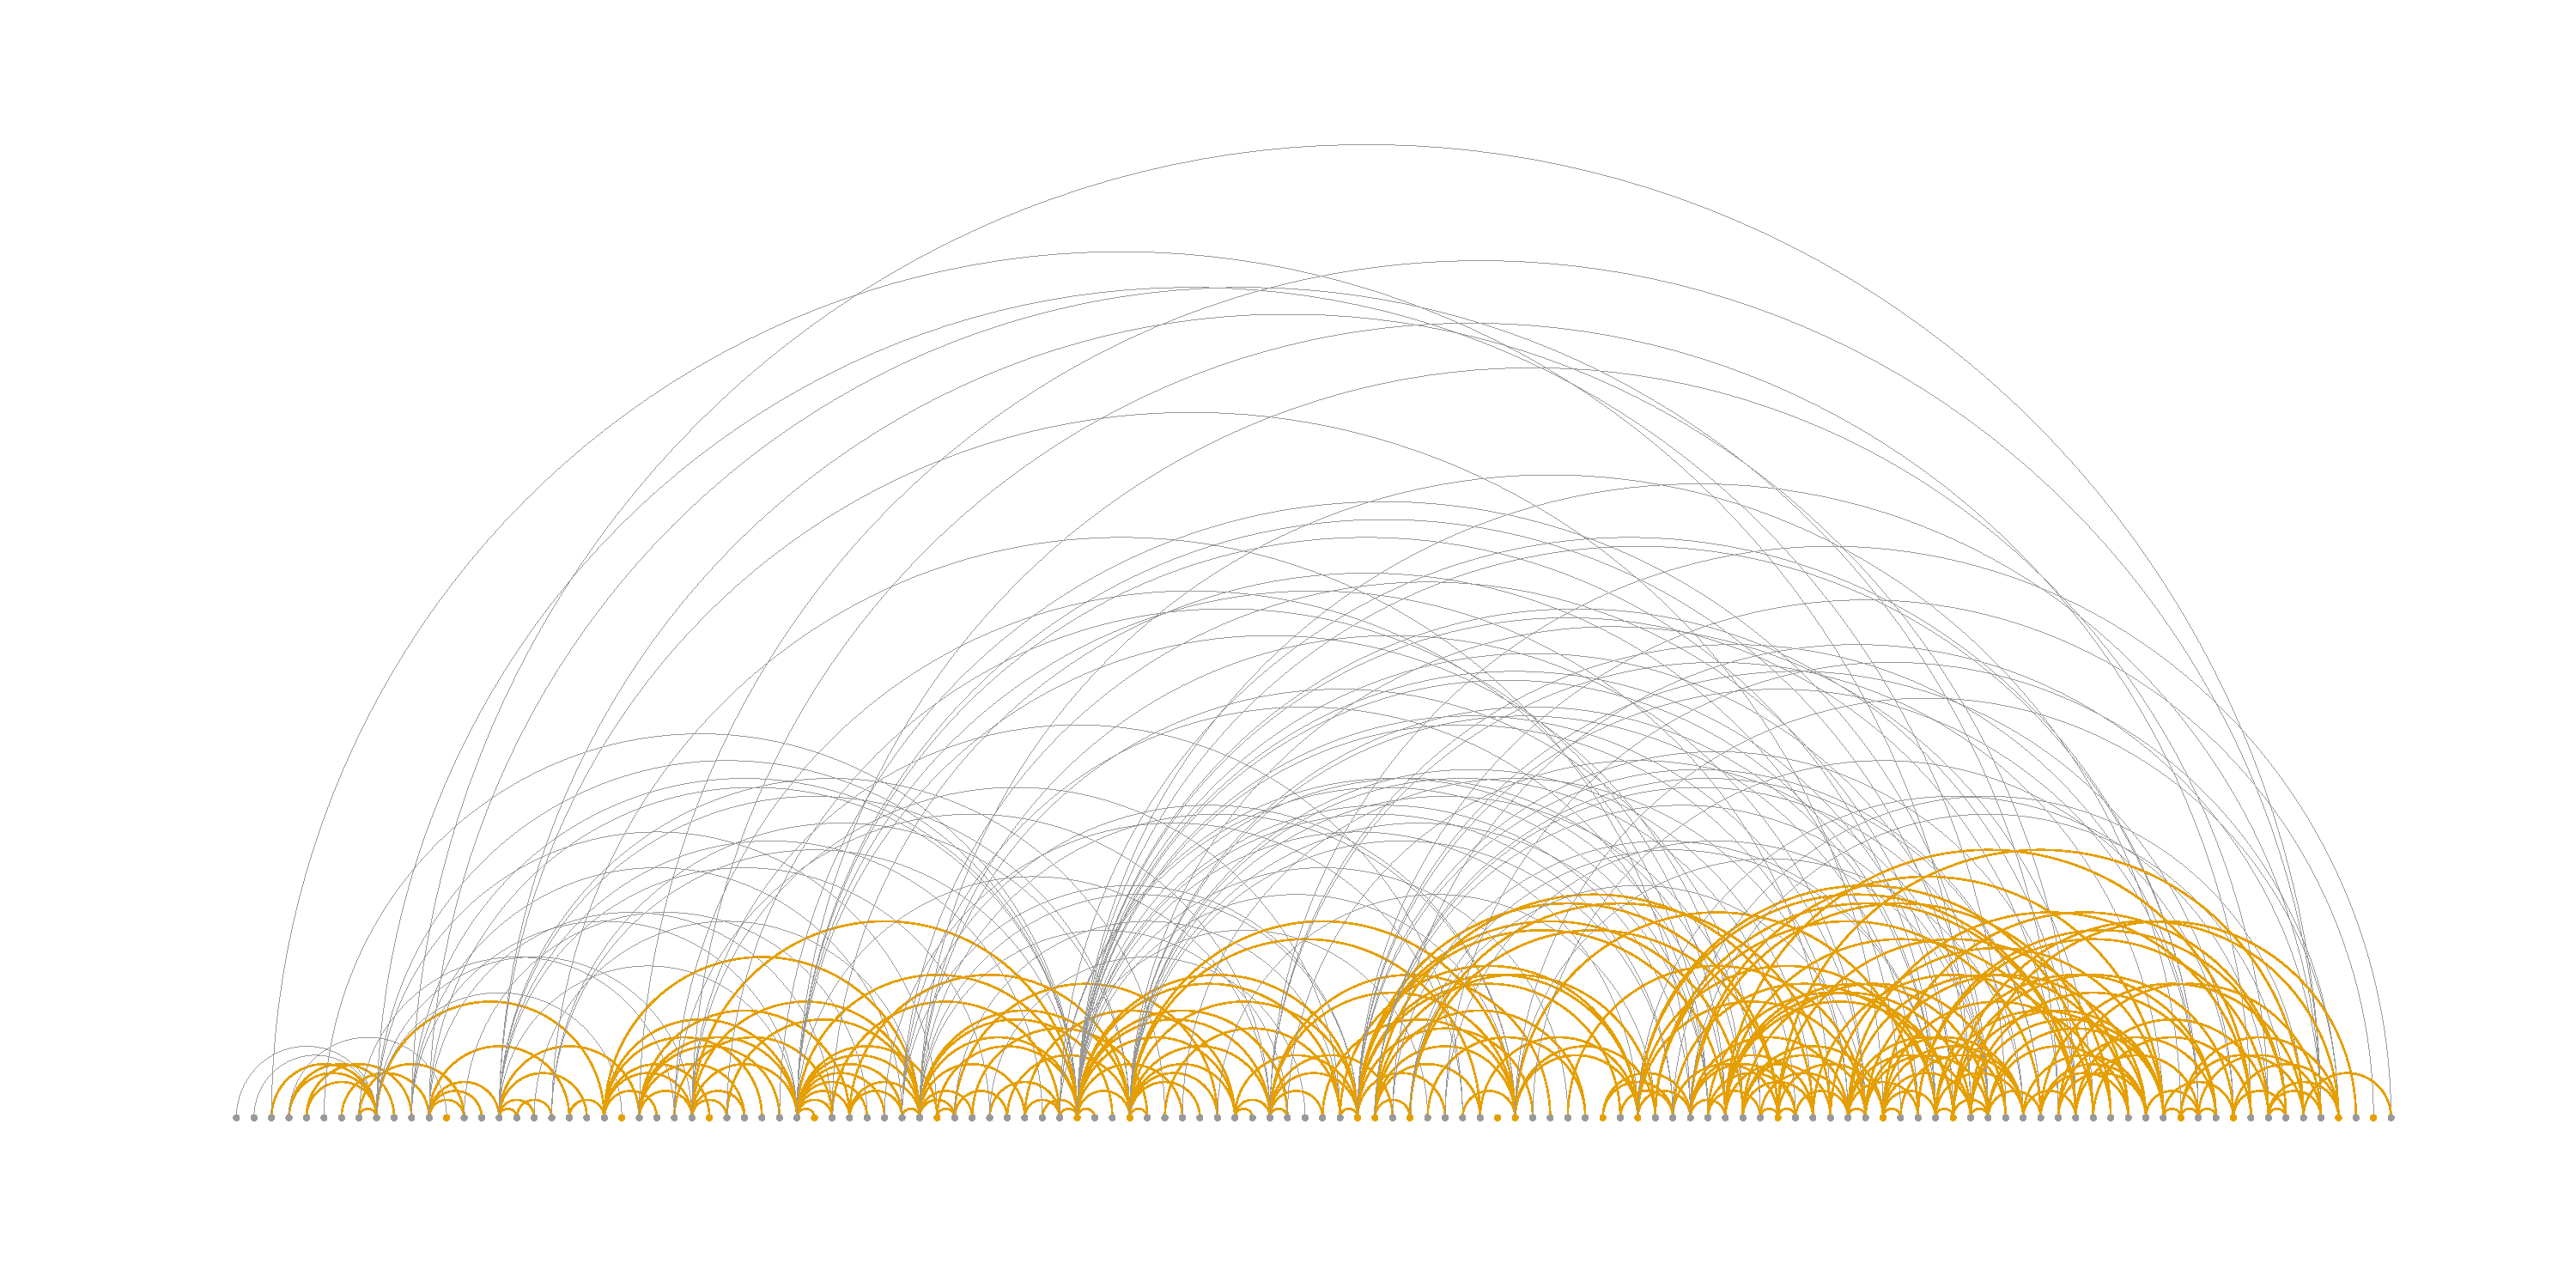
\includegraphics[width=\textwidth]{images/arcdiagram}
\caption{Arc diagram of pre-text selection. Nodes represent years of publication observed in the collection. Arcs between two years $i$ and $j$ are created if a story from year $i$ selects a story from year $j$ as its pre-text. Arcs colored yellow represent time spans shorter than the mean time span; gray arcs represent time spans longer than the mean. A node colored yellow indicates that in its corresponding year at least one retelling selects a pre-text with the same year of publication as the retelling.}
\label{fig:arcdiagram}
\end{sidewaysfigure}

I take it to be a highly intriguing question whether and to what extent the evolutionary process of ``Red Riding Hood'', and children's literature in general, can also be explained under a neutral model of evolution in which retellers base their material on randomly selected retellings from previous generations. Under the neutral model, no single retelling of a story is more valuable than others, and whether or not a particular story element is adopted in a retelling is proportional to its popularity in previous generations. It is clear, however, that a neutral copying model does not suffice for explaining the strong preference for selecting temporally proximate pre-texts~\autocite[Cf.][]{Acerbi:2012id}. While under the neutral model, any retelling can become the dominant pre-text for further retelling, the present study has clearly shown the need for a mechanism that explains the age-bias for selecting more recently produced versions.

Interestingly, the apparent age-bias (as represented by the discovered gamma-distributed selection of pre-texts with a strong lopsidedness towards texts in temporal proximity) could be interpreted as a kind of `cultural amnesia'. Figure \ref{fig:arcdiagram} presents an alternative visualization of this gamma distribution. In this so-called `arc diagram', nodes represent years of publication observed in the collection. Arcs between two years $i$ and $j$ are created if a story from year $i$ selects a story from year $j$ as its pre-text. Arcs colored yellow represent time spans shorter than the mean time span; gray arcs represent time spans longer than the mean. A node colored yellow indicates that in its corresponding year at least one retelling selects a pre-text with the same year of publication as the retelling. The gamma distribution, then, resembles a kind of `memory parameter'. It is an interesting question how this memory parameter influences the rate of change of a cultural artifact~\autocite[Cf.][]{Perreault:2012}. One might hypothesize that with an increasing number of possible generations to sample from, the rate of change decreases. With more generations, it is more difficult for an innovation to `catch on' because its likelihood of being selected is reduced. This inhibiting effect of a larger (textual) community on change is addressed by \citeauthor{Anderson:2000} in the context of oral culture:
\begin{quotation}
    \noindent ``[I]f details become sufficiently well fixed, generations of storytellers and listeners in an oral culture will automatically correct them a good deal of the time. A brilliant parody of the mischievous grandfather attempting to tell wrong versions of a well-known fairytale furnishes all the proof that is needed: the child will not tolerate a tale of `Little Green Riding Hood' going through the wood and meeting a giraffe, or meeting a wolf that asks `what's ten times eight?'.''\autocite[19]{Anderson:2000}
\end{quotation}
Although it is doubtful whether a child will indeed not tolerate such a story, she will immediately recognize it to be a retelling of ``Red Riding Hood'', which essentially proves the same point. 

\citeauthor{bentley:2011} study the effect of such a memory parameter in the context of the neutral model of evolution~\autocite{bentley:2011}. They generalize the neutral model by adding a memory parameter $m$. This parameter controls how many generations an individual is allowed to look back in time, ranging from only the immediate previous generation ($m=1$) to all generations ($m=\textrm{all}$). In the case of $m=1$ the model is equivalent to the `traditional' random copying model. In the special case of $m=\textrm{all}$, cultural traits do not go extinct. \citeauthor{bentley:2011} show that increasing $m$ reduces the effect of the innovation rate parameter, and hence has an inhibiting effect on cultural change. Furthermore, they show that adding more generations to the sample space has a conservative effect on the replacement of words in the vocabulary of languages~\autocite{bentley-comment:2011}. In the memory-parameterized neutral model, individuals randomly select an individual to copy from using a uniform distribution over $m$ previous generations. The memory-parameterized model by \citeauthor{bentley:2011} is essentially useful, but, as the present study has shown, a uniform distribution over $m$ previous generations might be too simplistic to account for all processes of cultural change. Because of its simplicity, however, the memory-parameterized model can easily be modified so that it accounts for more skewed distributions in which age acts as a bias in selection.

Simple, idealized models of cultural change, such as the memory-parameterized neutral model, allow researchers to abstract away from idiosyncratic properties of a particular case under investigation, and apply it to both children's literature at large as well as cultural change in general. The age-dependent selection in the transmission of ``Red Riding Hood'' also emerges in examples from biology~\autocite[E.g.][]{Grunst:2014} and ties in with other studies in cultural evolution investigating fashion trends~\autocite[E.g.][]{Acerbi:2012id,kandler:2015,Mauch:2015ix}. It would be interesting to further test whether the hypothesis that pre-texts in children's literature tend to come from the recent past, and subsequently examine whether there is a different age-bias in the transmission of other textual genres or cultural artifacts. One of the most important assets of the cultural evolutionary modeling approach, then, is that it enables researchers to explore parsimonious mechanisms and generic explanations that intersect such diverse examples of cultural change.

It should be stressed that age-bias does not fully account for the differential fitness of story variants. The preference for temporally proximate pre-texts alone cannot explain why authors choose for one or another retelling from the same time period. To arrive at such insights, then, we should consider ``a longish list of psychological, social, and ecological processes that interact to generate the differential ``fitness'' of cultural variants''~\autocite{Henrich:2008}. For instance, the growing disapproval of violence in the poetics of children's stories may have impacted the choices made by retellers (e.g.\ within the group of temporally proximate retellings, non-violent versions may thus display a transmission advantage over more violent ones). If such socio-cultural factors co-generate differential fitness with age-dependent selection, then the combination of these factors should yield a model of cultural change that accurately reflects the mechanisms underlying the selection of pre-texts.

In my final words, I would like to draw attention to the collection of Dutch ``Red Riding Hood'' retellings presented in this study. I believe that this collection, which consists of half a million words of ``Red Riding Hood'' and spans a time period of more than two hundred years, forms a small, yet unique and highly specialized collection that will hold potential for a variety of research activities to all those engaged in the study of children's literature, folkloristics, linguistics and cultural evolution. One may assume that the texts in the collection target a homogeneous audience and generally tell the same abstract content over and over. Characteristics as these allow researchers to study aspects of micro-variation, linguistic change, literary developments and cultural evolution that are otherwise deemed less attainable.